%  A simple AAU report template.
%  2015-05-08 v. 1.2.0
%  Copyright 2010-2015 by Jesper Kjær Nielsen <jkn@es.aau.dk>
%
%  This is free software: you can redistribute it and/or modify
%  it under the terms of the GNU General Public License as published by
%  the Free Software Foundation, either version 3 of the License, or
%  (at your option) any later version.
%
%  This is distributed in the hope that it will be useful,
%  but WITHOUT ANY WARRANTY; without even the implied warranty of
%  MERCHANTABILITY or FITNESS FOR A PARTICULAR PURPOSE.  See the
%  GNU General Public License for more details.
%
%  You can find the GNU General Public License at <http://www.gnu.org/licenses/>.
%
%  A simple AAU report template.
%  2015-05-08 v. 1.2.0
%  Copyright 2010-2015 by Jesper Kjær Nielsen <jkn@es.aau.dk>
%
%  This is free software: you can redistribute it and/or modify
%  it under the terms of the GNU General Public License as published by
%  the Free Software Foundation, either version 3 of the License, or
%  (at your option) any later version.
%
%  This is distributed in the hope that it will be useful,
%  but WITHOUT ANY WARRANTY; without even the implied warranty of
%  MERCHANTABILITY or FITNESS FOR A PARTICULAR PURPOSE.  See the
%  GNU General Public License for more details.
%
%  You can find the GNU General Public License at <http://www.gnu.org/licenses/>.
%
\documentclass[11pt,twoside,a4paper,openright]{report}
%%%%%%%%%%%%%%%%%%%%%%%%%%%%%%%%%%%%%%%%%%%%%%%%
% Language, Encoding and Fonts
% http://en.wikibooks.org/wiki/LaTeX/Internationalization
%%%%%%%%%%%%%%%%%%%%%%%%%%%%%%%%%%%%%%%%%%%%%%%%
% Select encoding of your inputs. Depends on
% your operating system and its default input
% encoding. Typically, you should use
%   Linux  : utf8 (most modern Linux distributions)
%            latin1 
%   Windows: ansinew
%            latin1 (works in most cases)
%   Mac    : applemac
% Notice that you can manually change the input
% encoding of your files by selecting "save as"
% an select the desired input encoding. 
\usepackage[utf8]{inputenc}
% Make latex understand and use the typographic
% rules of the language used in the document.
\usepackage[english, frenchb]{babel}
% Use the palatino font
\usepackage[sc]{mathpazo}
\linespread{1.05}         % Palatino needs more leading (space between lines)
% Choose the font encoding
\usepackage[T1]{fontenc}
%%%%%%%%%%%%%%%%%%%%%%%%%%%%%%%%%%%%%%%%%%%%%%%%
% Graphics and Tables
% http://en.wikibooks.org/wiki/LaTeX/Importing_Graphics
% http://en.wikibooks.org/wiki/LaTeX/Tables
% http://en.wikibooks.org/wiki/LaTeX/Colors
%%%%%%%%%%%%%%%%%%%%%%%%%%%%%%%%%%%%%%%%%%%%%%%%
% load a colour package
\usepackage{xcolor}
\definecolor{aaublue}{RGB}{33,26,82}% dark blue
% The standard graphics inclusion package
\usepackage{graphicx}
% Set up how figure and table captions are displayed
\usepackage{caption}
\captionsetup{%
  font=footnotesize,% set font size to footnotesize
  labelfont=bf % bold label (e.g., Figure 3.2) font
}
% Make the standard latex tables look so much better
\usepackage{array,booktabs}
% Enable the use of frames around, e.g., theorems
% The framed package is used in the example environment
\usepackage{framed}

%%%%%%%%%%%%%%%%%%%%%%%%%%%%%%%%%%%%%%%%%%%%%%%%
% Mathematics
% http://en.wikibooks.org/wiki/LaTeX/Mathematics
%%%%%%%%%%%%%%%%%%%%%%%%%%%%%%%%%%%%%%%%%%%%%%%%
% Defines new environments such as equation,
% align and split 
\usepackage{amsmath}
% Adds new math symbols
\usepackage{amssymb}
% Use theorems in your document
% The ntheorem package is also used for the example environment
% When using thmmarks, amsmath must be an option as well. Otherwise \eqref doesn't work anymore.
\usepackage[framed,amsmath,thmmarks]{ntheorem}

%%%%%%%%%%%%%%%%%%%%%%%%%%%%%%%%%%%%%%%%%%%%%%%%
% Page Layout
% http://en.wikibooks.org/wiki/LaTeX/Page_Layout
%%%%%%%%%%%%%%%%%%%%%%%%%%%%%%%%%%%%%%%%%%%%%%%%
% Change margins, papersize, etc of the document
\usepackage[
  inner=28mm,% left margin on an odd page
  outer=41mm,% right margin on an odd page
  ]{geometry}
% Modify how \chapter, \section, etc. look
% The titlesec package is very configureable
\usepackage{titlesec}
\titleformat{\chapter}[display]{\normalfont\huge\bfseries}{\chaptertitlename\ \thechapter}{20pt}{\Huge}
\titleformat*{\section}{\normalfont\Large\bfseries}
\titleformat*{\subsection}{\normalfont\large\bfseries}
\titleformat*{\subsubsection}{\normalfont\normalsize\bfseries}
%\titleformat*{\paragraph}{\normalfont\normalsize\bfseries}
%\titleformat*{\subparagraph}{\normalfont\normalsize\bfseries}

% Clear empty pages between chapters
\let\origdoublepage\cleardoublepage
\newcommand{\clearemptydoublepage}{%
  \clearpage
  {\pagestyle{empty}\origdoublepage}%
}
\let\cleardoublepage\clearemptydoublepage

% Change the headers and footers
\usepackage{fancyhdr}
\pagestyle{fancy}
\fancyhf{} %delete everything
\renewcommand{\headrulewidth}{0pt} %remove the horizontal line in the header
\fancyhead[RE]{\small\nouppercase\leftmark} %even page - chapter title
\fancyhead[LO]{\small\nouppercase\rightmark} %uneven page - section title
\fancyhead[LE,RO]{\thepage} %page number on all pages
% Do not stretch the content of a page. Instead,
% insert white space at the bottom of the page
\raggedbottom
% Enable arithmetics with length. Useful when
% typesetting the layout.
\usepackage{calc}

%%%%%%%%%%%%%%%%%%%%%%%%%%%%%%%%%%%%%%%%%%%%%%%%
% Bibliography
% http://en.wikibooks.org/wiki/LaTeX/Bibliography_Management
%%%%%%%%%%%%%%%%%%%%%%%%%%%%%%%%%%%%%%%%%%%%%%%%
\usepackage[backend=bibtex,
  bibencoding=utf8
  ]{biblatex}
\addbibresource{bib/mybib}

%%%%%%%%%%%%%%%%%%%%%%%%%%%%%%%%%%%%%%%%%%%%%%%%
% Misc
%%%%%%%%%%%%%%%%%%%%%%%%%%%%%%%%%%%%%%%%%%%%%%%%
% Add bibliography and index to the table of
% contents
\usepackage[nottoc]{tocbibind}
% Add the command \pageref{LastPage} which refers to the
% page number of the last page
\usepackage{lastpage}
% Add todo notes in the margin of the document
\usepackage[
%  disable, %turn off todonotes
  colorinlistoftodos, %enable a coloured square in the list of todos
  textwidth=\marginparwidth, %set the width of the todonotes
  textsize=scriptsize, %size of the text in the todonotes
  ]{todonotes}

%%%%%%%%%%%%%%%%%%%%%%%%%%%%%%%%%%%%%%%%%%%%%%%%
% Hyperlinks
% http://en.wikibooks.org/wiki/LaTeX/Hyperlinks
%%%%%%%%%%%%%%%%%%%%%%%%%%%%%%%%%%%%%%%%%%%%%%%%
% Enable hyperlinks and insert info into the pdf
% file. Hypperref should be loaded as one of the 
% last packages
\usepackage{hyperref}
\hypersetup{%
	pdfpagelabels=true,%
	plainpages=false,%
	pdfauthor={Author(s)},%
	pdftitle={Title},%
	pdfsubject={Subject},%
	bookmarksnumbered=true,%
	colorlinks=false,%
	citecolor=black,%
	filecolor=black,%
	linkcolor=black,% you should probably change this to black before printing
	urlcolor=black,%
	pdfstartview=FitH%
}% package inclusion and set up of the document
% see, e.g., http://en.wikibooks.org/wiki/LaTeX/Formatting#Hyphenation
% for more information on word hyphenation
\hyphenation{ex-am-ple hy-phen-a-tion short}
\hyphenation{long la-tex}% 
%  A simple AAU report template.
%  2015-05-08 v. 1.2.0
%  Copyright 2010-2015 by Jesper Kjær Nielsen <jkn@es.aau.dk>
%
%  This is free software: you can redistribute it and/or modify
%  it under the terms of the GNU General Public License as published by
%  the Free Software Foundation, either version 3 of the License, or
%  (at your option) any later version.
%
%  This is distributed in the hope that it will be useful,
%  but WITHOUT ANY WARRANTY; without even the implied warranty of
%  MERCHANTABILITY or FITNESS FOR A PARTICULAR PURPOSE.  See the
%  GNU General Public License for more details.
%
%  You can find the GNU General Public License at <http://www.gnu.org/licenses/>.
%
%
%
% see, e.g., http://en.wikibooks.org/wiki/LaTeX/Customizing_LaTeX#New_commands
% for more information on how to create macros

%%%%%%%%%%%%%%%%%%%%%%%%%%%%%%%%%%%%%%%%%%%%%%%%
% Macros for the titlepage
%%%%%%%%%%%%%%%%%%%%%%%%%%%%%%%%%%%%%%%%%%%%%%%%
%Creates the aau titlepage
\newcommand{\aautitlepage}[3]{%
  {
    %set up various length
    \ifx\titlepageleftcolumnwidth\undefined
      \newlength{\titlepageleftcolumnwidth}
      \newlength{\titlepagerightcolumnwidth}
    \fi
    \setlength{\titlepageleftcolumnwidth}{0.5\textwidth-\tabcolsep}
    \setlength{\titlepagerightcolumnwidth}{\textwidth-2\tabcolsep-\titlepageleftcolumnwidth}
    %create title page
    \thispagestyle{empty}
    \noindent%
    \begin{tabular}{@{}ll@{}}
      \parbox{\titlepageleftcolumnwidth}{
        \iflanguage{danish}{%
          
\includegraphics[width=\titlepageleftcolumnwidth]{figures/aau_logo_da}
        }{%
          
\includegraphics[width=\titlepageleftcolumnwidth]{figures/aau_logo_en}
        }
      } &
      \parbox{\titlepagerightcolumnwidth}{\raggedleft\sf\small
        #2
      }\bigskip\\
       #1 &
      \parbox[t]{\titlepagerightcolumnwidth}{%
      \textbf{Abstract:}\bigskip\par
        \fbox{\parbox{\titlepagerightcolumnwidth-2\fboxsep-2\fboxrule}{%
          #3
        }}
      }\\
    \end{tabular}
    \vfill
    \iflanguage{danish}{%
      \noindent{\footnotesize\emph{Rapportens indhold er frit tilgængeligt, men offentliggørelse (med kildeangivelse) må kun ske efter aftale med forfatterne.}}
    }{%
      \noindent{\footnotesize\emph{The content of this report is freely available, but publication (with reference) may only be pursued due to agreement with the author.}}
    }
    \clearpage
  }
}

%Create english project info
\newcommand{\englishprojectinfo}[8]{%
  \parbox[t]{\titlepageleftcolumnwidth}{
    \textbf{Title:}\\ #1\bigskip\par
    \textbf{Theme:}\\ #2\bigskip\par
    \textbf{Project Period:}\\ #3\bigskip\par
    \textbf{Project Group:}\\ #4\bigskip\par
    \textbf{Participant(s):}\\ #5\bigskip\par
    \textbf{Supervisor(s):}\\ #6\bigskip\par
    \textbf{Copies:} #7\bigskip\par
    \textbf{Page Numbers:} \pageref{LastPage}\bigskip\par
    \textbf{Date of Completion:}\\ #8
  }
}

%Create danish project info
\newcommand{\danishprojectinfo}[8]{%
  \parbox[t]{\titlepageleftcolumnwidth}{
    \textbf{Titel:}\\ #1\bigskip\par
    \textbf{Tema:}\\ #2\bigskip\par
    \textbf{Projektperiode:}\\ #3\bigskip\par
    \textbf{Projektgruppe:}\\ #4\bigskip\par
    \textbf{Deltager(e):}\\ #5\bigskip\par
    \textbf{Vejleder(e):}\\ #6\bigskip\par
    \textbf{Oplagstal:} #7\bigskip\par
    \textbf{Sidetal:} \pageref{LastPage}\bigskip\par
    \textbf{Afleveringsdato:}\\ #8
  }
}

%%%%%%%%%%%%%%%%%%%%%%%%%%%%%%%%%%%%%%%%%%%%%%%%
% An example environment
%%%%%%%%%%%%%%%%%%%%%%%%%%%%%%%%%%%%%%%%%%%%%%%%
\theoremheaderfont{\normalfont\bfseries}
\theorembodyfont{\normalfont}
\theoremstyle{break}
\def\theoremframecommand{{\color{gray!50}\vrule width 5pt \hspace{5pt}}}
\newshadedtheorem{exa}{Example}[chapter]
\newenvironment{example}[1]{%
		\begin{exa}[#1]
}{%
		\end{exa}
}% my new macros
\usepackage{float}
\usepackage{url}
\usepackage{listings}

\begin{document}
%frontmatter
\pagestyle{empty} %disable headers and footers
\pagenumbering{roman} %use roman page numbering in the frontmatter
\setcounter{secnumdepth}{3} % pour sous sous partie
%  A simple AAU report template.
%  2015-05-08 v. 1.2.0
%  Copyright 2010-2015 by Jesper Kjær Nielsen <jkn@es.aau.dk>
%
%  This is free software: you can redistribute it and/or modify
%  it under the terms of the GNU General Public License as published by
%  the Free Software Foundation, either version 3 of the License, or
%  (at your option) any later version.
%
%  This is distributed in the hope that it will be useful,
%  but WITHOUT ANY WARRANTY; without even the implied warranty of
%  MERCHANTABILITY or FITNESS FOR A PARTICULAR PURPOSE.  See the
%  GNU General Public License for more details.
%
%  You can find the GNU General Public License at <http://www.gnu.org/licenses/>.
%
\pdfbookmark[0]{Front page}{label:frontpage}%
\begin{titlepage}
  \addtolength{\hoffset}{0.5\evensidemargin-0.5\oddsidemargin} %set equal margins on the frontpage - remove this line if you want default margins
  \noindent%
  \begin{tabular}{@{}p{\textwidth}@{}}
    \toprule[2pt]
    \midrule
    \vspace{0.2cm}
    \begin{center}
    \Huge{\textbf{
      Etude expérimentale : déploiement IPv6% insert your title here
    }}
    \end{center}
    \begin{center}
      \Large{
        - adressage, autoconfiguration, routage, ICMPv6, QoS -% insert your subtitle here
      }
    \end{center}
    \vspace{0.2cm}\\
    \midrule
    \toprule[2pt]
  \end{tabular}
  \vspace{4 cm}
  \begin{center}
    {\large
      Rapport de projet SR04%Insert document type (e.g., Project Report)
    }\\
    \vspace{0.2cm}
    {\Large
      Grégoire Martinache\\
      Théo Bocquelet\\
      Minh Tri L\^{e}\\
      Augustin De Champs
      %Insert your group name or real names here
    }
  \end{center}
  \vfill
  \begin{center}
  Université de Technologie de Compiègne\\
  Génie Informatique
  \end{center}
\end{titlepage}
\clearpage
\cleardoublepage
\pdfbookmark[0]{Contents}{label:contents}
\pagestyle{fancy} %enable headers and footers again
\tableofcontents

%mainmatter
\pagenumbering{arabic} %use arabic page numbering in the mainmatter
\chapter{La couche réseau}\label{ch:couchereseau}

\section{Présentation de la couche réseau}

	\subsection{Rôles et services}

		Le rôle de la couche réseau est d’acheminer efficacement des paquets d’une source vers une destination suivant un parcours. Ce parcours peut être composé d’étapes intermédiaires. La couche réseau doit déterminer le meilleur chemin à prendre pour acheminer les paquets et doit donc connaître la topologie du réseau. Les réseaux peuvent avoir des protocoles différents, ce qui est un élément important à prendre en compte lors de la conception de la couche réseau.
        \medskip
        
		Un tel rôle demande un système de routage (\ref{ch:routage}) et d’adressage performant pour diriger les paquets entrants vers leur prochaine destination et doit tenir compte du réseau en lui-même (topologie, panne, surcharge, …). Il faut donc considérer les problèmes de congestion et plus généralement, la qualité de service (QoS : \ref{ch:qos}). 
        \medskip
        
		La couche réseau doit aussi tenir compte des besoins de l’application (type de service, fiabilité, …). Selon le besoin, il faut choisir entre le mode non connecté et le mode connecté : 
        \begin{itemize}
        \item Soit les paquets sont émis et routés indépendamment les uns des autres : les paquets sont nommés datagramme et le réseau est donc un réseau de datagramme.
		\item Si une connexion avec le destinataire est établie avant le début de la transmission, cette connexion est appelée circuit virtuel et le réseau est un réseau de circuit virtuel.
        \end{itemize}
        
			\begin{table}[H]
			\centering
			\label{MNC_MC}
			\begin{tabular}{|p{4cm}|p{5cm}|p{5cm}|}
			\hline
			\textbf{Aspect}               & \textbf{Datagrammes}                                                             & \textbf{Circuits virtuels (CV)}                                                                  \\ \hline
			Phase d'établissement         & Non nécessaire                                                                   & Requise                                                                                          \\ \hline
			Adressage                     & Chaque paquet contient les adresses complètes de la source et de la destination. & Chaque connexion requiert des informations d'identification de circuit dans la table de routage. \\ \hline
			Routage                       & Chaque paquet est routé indépendamment.                                          & La route est choisie lors de l'établissement du CV et suivie par tous les paquets.               \\ \hline
			Impact d'une panne de routeur & Aucun, excepté pour les paquets perdus au moment de l'incident.                  & Tous les CV passant par le routeur sont supprimés.                                               \\ \hline
			Qualité de service (QoS)      & Difficile à garantir                                                             & Facile à garantir si suffisamment de ressources peuvent être allouées par avance pour chaque CV. \\ \hline
			Contrôle de congestion        & Difficile.                                                                       & Facile si suffisamment de ressources peuvent être allouées par avance pour chaque CV             \\ \hline
			\end{tabular}
			\caption{Comparaison de réseaux de datagrammes et de réseaux de circuits virtuels \cite{Tanenbaum2003}}
			\end{table}
        %\medskip
       
		La couche réseau rend service à la couche transport et utilise la couche liaison.
		Elle rajoute un en-tête au segment de la couche transport puis fragmente si besoin le paquet pour la couche liaison. Il faut impérativement indépendance entre technologies de routeur et services pour assurer la maintenabilité et compatibilité.

	\subsection{Composition}
Pour assurer ses rôles, la couche réseau utilise une table de routage pour l’adressage et des algorithmes de routage pour le choix de la prochaine destination. 
	\newline
		La couche réseau utilise le protocole IP dans l'Internet qui est un protocole en mode non connecté. IPv4 et IPv6 (\ref{ch:ipv6}) sont deux versions de ce protocole. Nous étudierons la version IPv6 qui utilise le protocole ICMPv6 (\ref{ch:icmpv6}).
\chapter{Le routage}\label{ch:routage}
 
  \section{Présentation}
Le routage est le mécanisme qui gère les tables de routage et choisit l’itinéraire à suivre dans le réseau afin d’acheminer des paquets. Le routage peut se faire vers un ou plusieurs destinataires (multicast : \ref{sc:rout_multicast}) en utilisant un algorithme de routage approprié.

  \subsection{Algorithme de routage}
L’algorithme de routage décide du routage à suivre pour les paquets entrants et gère les tables de routage. 
\medskip

L’algorithme de routage doit être apte à s’adapter à toutes variations du réseau (défaillance matérielle et logicielle, modification rapide de la topologie du réseau, congestion). Il doit se montrer efficace au niveau local et global (maximiser l’efficacité globale peut être opposé à maximiser l’efficacité locale) et doit donc faire des compromis.
\\
Un algorithme de routage peut être statique ou dynamique. 
Dans le cas dynamique, l’algorithme construit la table de routage automatiquement en échangeant des informations au sein du réseau alors que dans le cas statique, la table doit être implémentée et modifiée manuellement.
\medskip

Nous nous intéresserons aux algorithmes de routage dynamiques, en particulier, le routage par vecteur de distance et le routage par informations d’état de lien. 

  \subsubsection{Routage par vecteur de distance (Distance vector)}\label{sc:rout_vect}
Le routage par vecteur de distance fonctionne par le principe de collaboration entre routeurs directement voisins. Chaque routeur a une table de routage contenant l’adresse de l’émetteur et du destinataire et le coût associé (dépend de plusieurs paramètres : nombre de saut, degré de congestion, temps de transit estimé). Les routeurs vont communiquer périodiquement (hello-time) le contenu de leur table de routage (update).

\begin{figure}[h]
    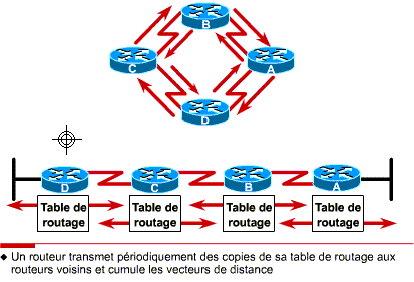
\includegraphics[width=270px]{figures/routage_vect.png}
    \centering
    \caption{Routage par vecteur de distance \cite{Rout_vecteur}}
    \end{figure}

Le routeur va ainsi pouvoir actualiser sa table de routage et prendre en compte les modifications du réseau (nouvelles destinations, coût modifié, panne).
\medskip

Suivant la destination qu’un paquet doit prendre, le routeur va consulter sa table de routage et emprunter la destination au coût le plus faible. Ainsi, la distance pour arriver à destination est calculée pas à pas et le routeur n’a pas connaissance de la topologie entière du réseau.
\medskip

Les désavantages des protocoles à vecteurs de distance sont :

	\begin{itemize}
	\item La charge réseau par les updates
    \item Le délai de convergence 15: un délai non négligeable est nécessaire pour savoir qu’un voisin est définitivement déconnecté (panne ou non). 
    \\
    Cet algorithme n’est donc pas efficace pour gérer un réseau à la topologie non stable.
    \item La latence : un certain délai est nécessaire pour actualiser la table de routage si le réseau est grand.
	\end{itemize}

  \subsubsection{Routage par informations d’état de lien (Link State)}\label{sc:rout_lien}
Contrairement à l’algorithme précédent, le routage par informations d’état de lien va chercher à comprendre la topologie complète du réseau, ce qui répond aux limitations du routage vecteur de distance.
\\
Cet algorithme se déroule en cinq points :
\begin{itemize}
\item Découverte des voisins du routeur : communique avec les voisins directs afin d’obtenir leur adresse et prise en compte des LAN à diffusion (réseau diffusant une information à tous les routeurs connectés du LAN) où il est seulement nécessaire de connaître une adresse du LAN.
\item Définition des coûts de lien : associe une adresse à un coût qui dépend de la distance, du débit et temps de transit estimé afin de trouver le chemin le plus optimal (au coût moindre).
\item Élaboration des paquets d’états de lien : Dès que le routeur possède les informations nécessaires sur ses voisins, il transmet un paquet d’états de lien à tous ses voisins qui renseigne l’état du réseau à proximité direct du routeur.
\\
Le paquet contient l’adresse de l’émetteur, un numéro de séquence, un âge, et l’adresse de ses voisins associés à leur coût. Il faut aussi décider de la fréquence d’envoi de ces paquets (par période fixe ou lors d’une modification du réseau).
\item Distribution des paquets d’états de lien : Assure l’envoi et la réception des paquets d’états de lien à tous les routeurs, et rapidement. Cette étape gère les numéros de séquence ainsi que l’âge des paquets afin d’éviter toute duplication.
\item Calcul de nouvelles routes : Dès que le routeur a reçu tous les paquets d’états de lien, il va pouvoir représenter le réseau dans son ensemble par un graphe. Ensuite, il suffit d’appliquer l’algorithme de Dijkstra sur le graphe qui va calculer le plus court chemin.
\end{itemize}
\medskip

Le principal désavantage de cet algorithme est qu’il est gourmand en capacité mémoire (chaque routeur a connaissance du réseau en entier) et calcul (il faut régulièrement calculer le plus court chemin du graphe).
Cependant, il est réactif aux variations du réseau.


  \section{Les protocoles de routage}
Nous allons traiter deux protocoles de routage intradomaine (protocole de passerelle intérieure) très répandus. 

  \subsection{Le protocole RIP (RIPng : Routing Information Protocol)}\label{sc:ripng}
Le protocole de routage RIP se base sur le routage par vecteur de distance (\ref{sc:rout_vect}). De ce fait, il possède les mêmes défauts et fonctionne sous le même principe, mais introduit une limite de coût : 15, afin d’éviter les boucles de routage. RIPng inclut les masques sous-réseau dans les updates pour les réseaux qui en ont besoin (VLMS : Variable Length Masque Subnet).
\\
Il supporte l’IPv6.
\\
L’adresse multicast utilisée est \textit{224.0.0.9}.

    \begin{figure}[h]
    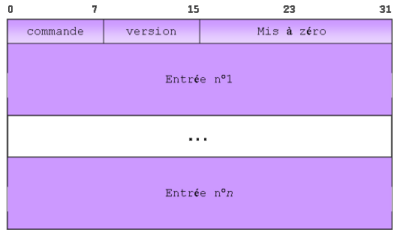
\includegraphics[width=270px]{figures/RIPvng_paquet.png}
    \centering
    \caption{Format d'un paquet RIPng \cite{Xripng}}
    \end{figure}

    \begin{figure}[H]
    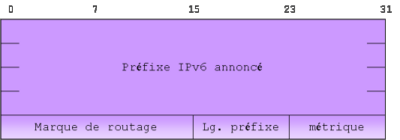
\includegraphics[width=270px]{figures/RIPvng_entree.png}
    \centering
    \caption{Champ entrée d'un paquet RIPng \cite{Xripng}}
    \end{figure}

Il n’est pas adapté aux grands réseaux.

  \subsection{Le protocole OSPF (OSPFv3 : Open Shortest Path First)}
Le protocole de routage OSPF se base sur le routage par état de lien (\ref{sc:rout_lien}). Il répond aux défauts du protocole RIP.
\\
Voici les services apportés par le protocole :
    \begin{itemize}

    \item Protocole ouvert donc non propriétaire.
    \item Routage par type de service : il est possible de spécifier un type de service dans les paquets.
    \item Permet la division du réseau en aires autonomes et indépendantes entre elles. L’interface entre deux aires est nommée l’aire backbone, ce qui permet d’optimiser le routage en communiquant des résumés de route ainsi que la nature des réseaux IP. Chaque routeur a donc connaissance de la topologie de son aire.
    \item Gère le routage machine-machine, vers réseaux et sous-réseaux.
    \item Utilise l’adressage multicast IP (voir \ref{sc:@multicast}).
    \item Réactif aux variations du réseau (panne, congestion…) et optimal : car basé sur le routage par état de lien. Il tient compte du trafic afin de ne pas envoyer tous les paquets sur la meilleure route et de ne pas délaisser les autres routes possibles.
    \item Peut évaluer une variété de types de coût (nombre de sauts, débit…). 
    \item Supporte VLMS (comme RIPng (\ref{sc:ripng})).
    \item Supporte l’IPv6 (voir \ref{ch:ipv6}).

    \end{itemize}
\medskip

OSPF utilise cinq types de messages différents :

\begin{figure}[H]
    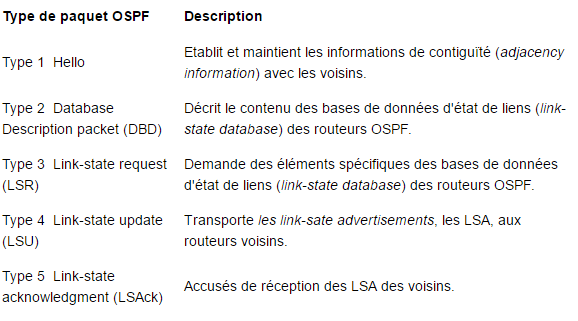
\includegraphics[width=340px]{figures/OSPF_type_paquet.PNG}
    \centering
    \caption{Type de paquet OSPF \cite{Xospf}}
    \end{figure}
    
Ce protocole est rapide, robuste aux variations du réseau, interopérable et permet de gérer des paramètres utiles à la QoS (\ref{ch:qos}) (répartition du trafic, prise en compte du type de service…).
\\
Il possède les mêmes défauts que le routage par état de lien (\ref{sc:rout_lien}), mais la répartition par aire complique la configuration.

  \section{Le routage multicast}\label{sc:rout_multicast}
  
  \subsection{Les besoins}
Une application requiert de diffuser des données en continu à un groupe particulier de personnes, comme le streaming vidéo en direct d’un concert et plus généralement, la téléconférence. Dans cet exemple, un émetteur unique transmet un flux d’information à un public visé. Pour ce faire, il faut utiliser le routage multicast.

  \subsection{Les difficultés}
Toute la difficulté du routage multicast réside dans la diffusion efficace de l’information au groupe concerné.
\\
Cela requiert donc un routage performant.
\\
L’efficacité de la diffusion dépend de deux cas de figure :
  \begin{itemize}
  \item Le groupe est dense : les membres du groupe sont dispersés sur une majeure partie du réseau.
  \item Le groupe n’est pas dense : beaucoup d’éléments du réseau ne font pas partie du groupe.
  \end{itemize}

  \subsection{Quelles solutions ?}
Pour communiquer à plusieurs membres particuliers du réseau, plusieurs techniques existent. Elles consistent toutes à obtenir le graphe du groupe de diffusion sans boucles (arbre du groupe) par élagage du graphe du réseau sans boucles (arbre recouvrant).

  \subsubsection{Avec un routage par état de lien}
Dans ce cas, la topologie complète du réseau est connue par chaque routeur. Il est ainsi facile de construire un graphe contenant le réseau sans les éléments qui ne sont pas membres du groupe ainsi que leurs liens.
\\
Cela permet d’obtenir un graphe spécifique au groupe de diffusion.

  \subsubsection{Avec un routage par vecteur de distance (DVMRP : Distance Vector Multicast Routing Protocol)}
  Cette solution se base sur le protocole RIP (\ref{sc:ripng}).
  \\
En trois étapes :
    \begin{itemize}
    \item Un premier message pour le groupe est envoyé sur le réseau. Le champ TTL (time to live) du message restreint la zone de diffusion de ce dernier.
    \item Tous les routeurs recevant ce message, mais ne faisant pas partie du groupe multicast et n’étant pas liés directement à un membre renvoient un message PRUNE à l’émetteur. Ce message précise qu'un routeur n’est pas membre du groupe et ne veut plus recevoir de message de ce groupe.
    \item À partir de la réponse de chacun des récepteurs, il est ainsi possible de construire un arbre du groupe multicast.
    \end{itemize}
\medskip

L’arbre obtenu ne contient que les liaisons utiles pour diffuser un message sur le groupe multicast. Il est donc efficace.
\\
Cependant, le problème est que cela nécessite une grande capacité de travail pour chaque routeur, en particulier dans les grands réseaux. En effet, il faut constituer et mémoriser un arbre pour chaque routeur membre du groupe dans un réseau de taille supérieur ou égal.

  \subsubsection{Avec la technique du coeur de l'arbre (CBT : Core-based tree)}
Dans ce cas, un seul arbre est calculé par groupe et chaque routeur membre en a connaissance.
\\
Le principe est de décider d’un routeur racine (membre du groupe) : le cœur. L’arbre obtenu par cette technique est le CBT.
\medskip

Le cœur doit d’abord constituer le CBT. Chaque membre envoie un paquet vers le cœur, ce qui permet d’obtenir la route entre le cœur et chaque membre du groupe. L’arbre du groupe a donc le cœur comme racine et tous ses membres en branches et feuilles.

\begin{figure}[h]
    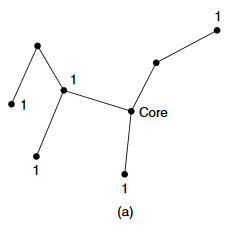
\includegraphics[width=160px]{figures/cbt.PNG}
    \centering
    \caption{Core-based tree}
    \end{figure}

Le choix de la racine est critique pour la performance.
\\
Cette technique est très optimale si le cœur est au milieu de l’arbre, et donc à distance plus ou moins égale de chaque membre du groupe. Elle se montre utile dans le cas où le groupe est dispersé dans le réseau.
\\
De plus, seul un arbre est nécessaire pour chaque membre du groupe et ceux qui ne sont pas membres du groupe ne travaillent pas. Ainsi, on gagne en capacité mémoire et calcul.
\chapter{Le protocole IPv6}\label{ch:ipv6}

\section{Présentation}
\subsection{Pourquoi l'IPv6 ?}
Le protocole IPv6 succède au protocole IPv4. Celui-ci a été conçu par l'Internet Enginnering Task Force (IETF) pour surmonter les manques de l'IPv4. L'IPv6 apporte notamment :
\begin{itemize}
\item Beaucoup plus d'adresses IP possibles  (avec un maximum de 667 millions de milliards d'appareils connectés sur chaque millimètre carré de la surface de la Terre !). 
    
    \begin{figure}[h]
    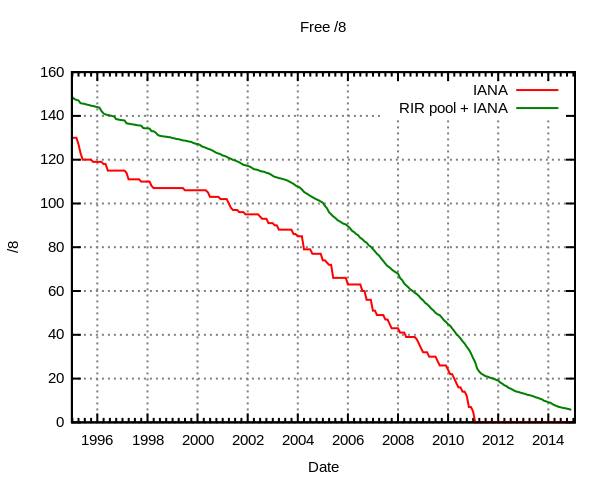
\includegraphics[width=250px]{figures/ipv4-exhaust.png}
    \centering
    \caption{Quantité d'adresse IPv4 disponibles au cours du temps}
    \end{figure}

\item L'implémentation directe de la Quality of Service (QoS \ref{ch:qos});
\item L'implémentation d'un protocole de sécurité (IPSec);
\item Le multicast;
\item La simplification de l'entête des paquets.
\end{itemize}


\subsection{Difficultés rencontrées}
L'IPv6 est incompatible avec l'IPv4 rendant compliqué son déploiement sur Internet. Les hôtes doivent donc proposer une \textit{double pile}, c'est à dire que les appareils disposent à la fois d'une adresse IPv4 et d'une IPv6.
    \begin{figure}[h]
    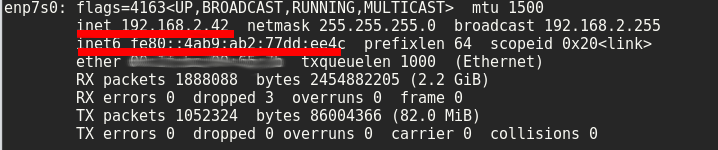
\includegraphics[width=250px]{figures/doubleStack.png}
    \centering
    \caption{Exemple de double pile sur mon ordinateur}
    \end{figure}
    
L'IPv6 étant une technologie encore jeune, les entreprises doivent également éduquer l'ensemble du personnel informatique ralentissant et compliquant la procédure de migration de IPv4 à IPv6 dans les grandes entreprises en plus de la rendre chère.

\section{Types d'adresses IPv6}

\begin{table}[!h]
  \centering
  \begin{tabular}{|l|l|} 
   \hline
    \textbf{Préfixe} & \textbf{Description} \\
    \hline
    ::/8 & Adresses réservées  \\
    \hline
    2000::/3 & Adresses unicast routables sur Internet  \\
    \hline    
    fc00::/7 & Adresses locales uniques  \\
    \hline    
    fe80::/10 & Adresses locales lien  \\
    \hline    
    ff00::/8 & Adresses multicast  \\
    \hline
  \end{tabular}
  \caption{Les différents types d'adresses IPv6.}
\end{table}
\textit{NB: On utilise la notation CIDR pour l'IPv6, de la même facon qu'avec l'IPv4.}

Nous allons désormais expliciter les différents types d'adresses ainsi que leurs utilitées.

\subsection{Les adresses réservées}

Certaines adresses IPv6 sont reservées pour une utilisation particulière : il en existe 13\cite{ReservedAddress}. On pourra noter les plus importantes :
\begin{table}[!h]
  \centering
  \begin{tabular}{|l|p{15cm}|} 
   \hline
    \textbf{Adresse} & \textbf{Description} \\
    \hline
    ::/128 & Adresse non spécifiée. Elle correspond à 0.0.0.0 en IPv4.  \\
    \hline
    ::1/128 & Boucle locale. Elle correspond à 127.0.0.1 en IPv4.  \\
    \hline
    2002::/16 & 6to4.\cite{6to4}. Mécanisme permettant d'envoyer des paquets IPv6 sur un réseau ne supportant que l'IPv4. \\
    \hline
    
  \end{tabular}
  \caption{Quelques adresses IPv6 réservées.}
\end{table}

\subsection{Les adresses unicast}
À la grande différence de l'adressage IPv4, il n'y a plus d'adresse de Broadcast (diffusion) en IPv6.
On pourra retrouver les adresses Unicast, Multicast et Anycast.\\

L' adresse Unicast sert à définir un hôte particulier. Un paquet émis avec cette adresse de destination n'est remis qu'à la machine ayant cette adresse IPv6.\\

IPv6 inclut deux assignations différentes d'adresses unicast :
\begin{itemize}
\item adresse unicast globale;
\item adresse lien local.
\end{itemize}
  
En IPv6, les adresses unicast se présentent ainsi :

\begin{table}[!h]
  \centering
  \begin{tabular}{|l|l|l|l|} 
   \hline
    \textbf{Champ} & Préfixe & Sous-réseau & Interface \\
    \hline
    \textbf{Bits} & \textit{48} & \textit{16} & \textit{64} \\
    \hline
  \end{tabular}
  \caption{Le format d'une adresse unicast. \cite{OracleUnicast}}
\end{table}

Les adresses en lien local sont toujours dans \textit{fc00::/7}.

\subsection{Les adresses multicast}\label{sc:@multicast}

L'adresse de Multicast concerne un ensemble d'hôtes appartenant à un même groupe de diffusion. Un paquet émis avec cette adresse de destination est remis à l'ensemble des machines concernées par cette adresse.\\

En IPv6, les adresses multicast se présentent ainsi :

\begin{table}[!h]
  \centering
  \begin{tabular}{|l|l|l|l|l|} 
   \hline
    \textbf{Champ} & Préfixe & Drapeau & Portée & Groupe \\
    \hline
    \textbf{Bits} & \textit{8} & \textit{4} & \textit{4} & \textit{112} \\
    \hline
  \end{tabular}
  \caption{Le format d'une adresse multicast. \cite{OracleMulticast}}
\end{table}

\subsection{Les adresses anycast}

L'adresse Anycast est ni plus ni moins de l'adressage multicast, à la différence qu'un paquet émis avec cette adresse de destination ne sera remis qu'à un seul membre du groupe. \\
Pour l'instant, une seule adresse anycast est définie et est réservée au routeur mais dans l'avenir, d'autres pourraient être définies. \\
La construction d'une adresse IPv6 anycast d'un sous-réseau (la seule définie actuellement) concatène le préfixe du sous réseau de l'interface et la valeur nulle pour la dernière partie de l'adresse.

\begin{table}[!h]
  \centering
  \begin{tabular}{|c|c|} 
   \hline
	\textit{n bits} & \textit{112 - nbits} \\
    \hline
    {Préfixe de sous-réseau} & {ID du groupe} \\
    \hline
  \end{tabular}
  \caption{Le format d'une adresse anycast.}
\end{table}

\chapter{Le protocole ICMPv6}\label{ch:icmpv6}

\section{Présentation}
\subsection{Qu'est-ce-qu'ICMP ?}

ICMP : Internet Control Message Protocol 
\medskip

ICMPv6 est l'un des protocoles fondamentaux d'Internet. Il permet aux routeurs d'envoyer des messages d'erreurs ou de contrôle à d'autres routeurs ou machines. Ces messages contiennent des informations sur les problèmes rencontrés lors de la transmission des paquets.
\medskip
    
Quelques exemples :
    \begin{itemize}
    	\item rapporter des erreurs trouvées dans le traitement de paquets
        \item effectuer des diagnostics
    \end{itemize}
\medskip

Les datagrammes ICMP sont transportés à l'intérieur de datagrammes IPv6 dans lequel un en-tête d'extension peut aussi être présent. Un message ICMP est identifié par sa valeur 58 positionnée dans le champ Next Header de l'en-tête IPv6. Le protocole ICMPv6 est implémenté au niveau de la couche 3.
\medskip

\begin{table}[!h]
  \centering
  \begin{tabular}{|l|l|l|} 
   \hline
   	Type & Code & Checksum \\
    \hline
    & Message Body &\\
    \hline
  \end{tabular}
  \caption{Format d'un message ICMPv6}
\end{table}

Champ \emph{type} : indique le type du message. Sa valeur détermine le format des données.

Champ \emph{code} : fournit des informations supplémentaires sur le type du message.

Champ \emph{checksum} : utilisé pour détecter une éventuelle corruption des données.

\subsection{Quelles sont les nouveautés apportées par ICMPv6 ?}

Quelques nouveautés :
	\begin{itemize}
    	\item suppression de certains types de messages devenus obsolètes
        \item renforcement de la sécurité des messages ICMP avec l'apparition du système d'authentification (Authentification Header) et de confidentialité (Encapsulating Security Payload Header) de IPv6
        \item ICMPv6 reprend des fonctionnalités qui étaient à la base implémentées dans d'autres protocoles pour IPv4, par exemple la découverte de voisin qui était effectuée par ARP
    \end{itemize}
\medskip

On peut aussi noter que le protocole ICMPv6 n'est pas seulement utilisé pour rapporter des erreurs mais implémente par exemple le mécanisme de découverte de route utilisé pour configurer les hôtes. Il est aussi utilisé pour le management des adresses multicast.
    
\medskip

\subsection{Détermination de l'adresse source d'un message}

Un noeud envoyant un message ICMPv6 doit déterminer à la fois les adresses IPv6 de source et de destination de l'en-tête IPv6 avant de calculer la somme de contrôle. Si le noeud a plus d'une adresse unicast, il doit choisir l'adresse source du message de la manière suivante :
    \begin{itemize}
		\item{si le message est une réponse à un message envoyé à l'une des adresses unicast du noeud, l'adresse source de la réponse doit être la même.}
		\item{si le message est une réponse à un message envoyé en multicast, ou anycast, d'un groupe dont le noeud est membre, l'adresse de la réponse doit appartenir au groupe.}
	\end{itemize}
    
\subsection{Traitement des messages ICMPv6}

Les règles suivantes sont appliquées pour traiter les messages ICMPv6 :
    \begin{list}{}{}
    	\item 1 : les messages d'erreur inconnus doivent être passés à la couche supérieure ayant causé le datagramme responsable de l'erreur
        \item 2 : les messages informatifs inconnus sont jetés
        \item 3 : un noeud IPv6 doit limiter le nombre de messages d'erreur qu'il envoie
        \item 4 : un message d'erreur ne doit jamais être envoyé en réponse à :
        	    \begin{itemize}
					\item un message d'erreur
					\item un message de redirection
                    \item un paquet destiné à une adresse multicast IPv6
                    \item un paquet dont l'adresse source identifie plusieurs noeuds
				\end{itemize}
    \end{list}
    
\section{Messages d'erreur}

On identifie les messages d’erreur grâce à la présence d’un 0 en bit de poids fort pour le type, cela représente donc les types de 0 à 127.
\medskip

Types de messages d'erreur ICMPv6 :         
    \begin{list}{}{}
    	\item 1 : Destination inatteignable
        \item 2 : Paquet trop grand 
        \item 3 : Temps écoulé
        \item 4 : Problème de paramètre
        \item 100 : Expérimentation privée
        \item 101 : Expérimentation privée
        \item 127 : Réservé pour la création de nouveaux messages d'erreur
    \end{list}
\medskip

Ces messages permettent d'effectuer des diagnostics, de savoir pourquoi le paquet n'a pas été acheminé, ou pourquoi il a été rejeté. Ils sont en rapport avec les problèmes de livraison des paquets IP.

Une fois reçu, ces messages sont délivrés soit aux processus utilisateurs, soit à un protocole de transport (exemple : TCP).

\subsection{Type 1 : destination inatteignable}

Les messages de ce type sont utilisés pour indiquer qu'un paquet a pu ne pas être délivré à son destinataire soit à cause d'un problème rencontré sur le chemin, soit à cause d'un manque d'intérêt du destinataire.

Ce message n'utilise pas le champ message body.
\medskip

Champ \emph{code} :
    \begin{list}{}{}
    	\item 0 : Pas de route vers la destination 
        \item 1 : Communication avec la destination interdite administrativement (firewall)
        \item 2 : La destination est hors de portée   
        \item 3 : Adresse inatteignable
        \item 4 : Port inatteignable 
        \item 5 : La politique de filtrage estime que le paquet n'est pas conforme
        \item 6 : Rejet de la route vers la destiantion
    \end{list}

\subsection{Type 2 : paquet trop grand}

Ce message utilise le champ message body pour y indiquer le MTU du noeud posant problème.
\medskip

Champ \emph{code} : il est mis à 0 par l'émetteur et ignoré par le récepteur.

Champ \emph{MTU} : contient la valeur du MTU du noeud qui a rejeté le paquet        

\subsection{Type 3 : temps dépassé}

Ce message est envoyé par un routeur lorsque la durée de vie d'un paquet est dépassée. 

Ce message n'utilise pas le champ message body.
\medskip

Champ \emph{code} :
    \begin{list}{}{}
    	\item 0 : Le "hop limit" est dépassé
        \item 1 : Temps de réassemblement des fragments dépassé
    \end{list}

\subsection{Type 4 : problème de paramètre}

Ce message ICMP est envoyé quand un paramètre dans un paquet reçu est invalide. 

Ce message utilise le champ message body pour y stocker un pointeur.
\medskip

Champ \emph{code} :           
    \begin{list}{}{}
    	\item 0 : Champ d'en-tête erroné
        \item 1 : En-tête suivant non reconnaissable
        \item 2 : Option IPv6 non reconnue  
    \end{list}

Champ \emph{pointeur} : identifie l'octet du paquet où l'erreur a été détectée. Le pointeur pointera au delà de la fin du paquet ICMPv6 si le champ erroné se trouve au delà de ce qui peut tenir dans un message d'erreur ICMPv6.

\section{Messages informatifs}

	On identifie les messages informatifs grâce à la présence d’un 1 en bit de poids fort pour le type, cela représente donc les types de 128 à 255.
\medskip

Types de messages informatifs ICMPv6 : 
    \begin{list}{}{}
    	\item 128 : Demande d'écho
        \item 129 : Réponse à un écho
        \item 200 : Expérimentation privée  
        \item 201 : Expérimentation privée  
        \item 255 : Réservée pour la création de nouveaux messages informatifs  
    \end{list}
\medskip

Les messages d'écho sont par exemple utilisés par l'utilitaire "ping", permettant de savoir si une machine est présente sur le réseau. Ils servent à tester la connexion entre deux points.

\begin{table}[!h]
  \centering
  \begin{tabular}{|l|l|l|} 
   \hline
   	Type & Code & Checksum \\
    \hline
    Identifiant & Numéro de séquence & \\
    \hline
    Données & & \\
    \hline
  \end{tabular}
  \caption{Format des message de demande et réponse d'écho \cite{}}
\end{table}

\subsection{Type 128 : demande d'écho}

Champ \emph{identifiant} : l'identifiant aide à faire correspondre les réponses d'écho aux demandes.

Champ \emph{numéro de séquence} : le numéro de séquence aide à faire correspondre les réponses d'écho aux demandes.    

Champ \emph{données} : contient des données à transmettre

\subsection{Type 129 : réponse d'écho}

Champ \emph{identifiant} : contient l'identifiant du message correspondant à la demande d'écho.

Champ \emph{numéro de séquence} : contient le numéro de séquence du message correspondant à la demande d'écho.   

Champ \emph{données} : contient des données provenant du message correspondant à la demande d'écho.
\medskip

Les messages de réponse d'écho doivent être passés au noeud qui a créé une demande d'écho. 
    
On peut noter qu'il n'y a pas de limitation à la quantité de données que l'on peut fournir dans des messages de demande d'écho ou de réponse.
\chapter{La qualité de service}\label{ch:qos}

\section{Présentation}

Les besoins de chaque flux de données peuvent être caractérisés par quatre principaux paramètres : la fiabilité (reliability) , le temps d'acheminement (delay), la gigue (jitter), et la bande passante (bandwidth).\\
Fiabilité  : quel est le taux de perte des paquets dans le réseau ?\\
Temps d'acheminement : quel est le temps d'acheminement des paquets de la source à la destination ?\\
Gigue : avec quelle régularité les paquets arrivent-ils au destinataire ?\\
Bande passante : quelle quantité d'information peut être transmise en un temps donné (débit) ?\\
    
Les besoins pour chaque paramètre dépendent de l'application :
\begin{table}[!h]
  \centering
  \begin{tabular}{|l|l|l|l|l|} 
   \hline
    Application & Fiabilité & Temps d'acheminement & Gigue & Bande passante \\
    \hline
    Email & Important & Faible & Faible & Faible\\
    \hline
    Transfert de fichier & Important & Faible & Faible & Moyen\\
    \hline
    Navigation web & Important & Moyen & Faible & Moyen\\
    \hline
    Connexion distante & Important & Moyen & Moyen & Faible\\
    \hline
    Audio à la demande & Faible & Faible & Important & Moyen\\
    \hline
    Vidéo à la demande & Faible & Faible & Important & Important\\
    \hline
    Téléphonie & Faible & Important & Important & Faible\\
    \hline
    Vidéoconférence & Faible & Important & Important & Important\\
    \hline
  \end{tabular}
  \caption{Exemples des besoins de différentes applications. \cite{Tanenbaum2003}}
\end{table}

C'est pourquoi il est important de faire de la qualité de service en fonction du type d'application visée.\\

Il existe différentes techniques pour obtenir une bonne QoS :\\

\begin{itemize}
\item Surapprovisionnement (overprovisioning) :

Il s'agit de disposer de plus de ressources (espace de stockage, bande passante, débit...) que nécessaire, afin que tous les paquets puissent transiter sans la moindre attente. Cette solution est simple mais extrêmement coûteuse à mettre en place. D'autres solutions moins coûteuses permettent généralement d'atteindre les objectifs de Qualité de Service fixés. \\
\item La mise en mémoire tampon (buffering) :

Il s'agit de stocker les paquets d'un flux chez le destinataire avant de les délivrer. Cette solution permet de réduire la gigue (on peut contrôler la vitesse d'arrivée des paquets au destinataire) mais augmente le temps d'acheminement de la source à la destination.\\

\item La régulation de flux (traffic shaping) :

Il s'agit ici d'imposer à l'émetteur de transmettre ses paquets à une vitesse régulière (constante). Cela permet de diminuer la congestion dans le réseau (on empêche une machine d'envoyer une grande quantité de paquets en une seule fois).\\ Dans un protocole en mode connecté, l'émetteur et le récepteur peuvent aussi convenir des paramètres des flux de données à échanger lors de l'établissement de la connexion. Lorsque le destinataire reçoit un flux, et si le flux respecte la convention établie, le destinataire s'engage à transmettre les données dans les temps. Cette technique s'appelle la limitation du flux (traffic policing).\\

\item L'algorithme du seau percé (leaky bucket, Turner, 1986) :

Dans un seau percé rempli d'eau, peu importe la quantité d'eau dans le seau, le débit sortant ne varie pas; et lorsque le seau est plein, l'eau excédentaire est perdue. Dans cet algorithme, les paquets arrivants sont stockés dans une structure de file à taille fixée. A chaque tick d'horloge et si la file n'est pas vide, un paquet est défilé et envoyé. Lorsque la file est pleine, un paquet arrivant est jeté. Cet algorithme permet de fluidifier des échanges irréguliers ou limiter le débit dans un réseau.\\

\item L'algorithme du seau à jetons (token bucket) :

Cet algorithme est similaire à l'algorithme du seau percé mais plus flexible. Le seau percé contient un certain nombre de jetons. Un jeton est généré chaque intervalle de temps jusqu'à un certain seuil maximum du nombre de jetons total. Chaque paquet peut consommer un jeton pour être immédiatement transmis. Lorsqu'il n'y a plus de jetons disponibles, les paquets sont stockés comme dans l'algorithme du seau percé mais ne seront jamais jetés (a priori). Cet algorithme permet de mieux réguler le trafic lorsque de grande quantité de données arrivent à un routeur.\\

\item La réservation de ressource :

L'idée ici est de prévoir un chemin pour un certain flux de données (on créé une sorte de circuit virtuel), et de réserver toutes les ressources nécessaires sur cette route afin de garantir une bonne qualité de service pour ce flux passant par cette route. On pourra réserver de la bande passante, de l'espace de stockage ou encore de la capacité CPU dans les routeurs par exemple.\\

\item Le contrôle d'admission :

Lorsqu'un routeur reçoit un flux, il doit décider selon ses ressources disponibles immédiatement, de l'accepter ou de le rejeter. Cependant cette décision est compliquée car elle dépend de nombreux paramètres donnés (ou non) par l'émetteur. De plus, tous les routeurs sur le chemin de l'émetteur au destinataire peuvent avoir leurs propres contraintes.\\
Une solution est que l'émetteur transmette au destinataire les paramètres qu'il voudrait négocier (dont il aurait besoin) : nous les nommerons spécifications du flux. Tous les routeurs sur le chemin peuvent les examiner et les modifier si besoin mais seulement en réduisant le flux. Lorsque les spécifications ont été examinées par toutes les machines du chemin, elles sont adoptées : l'émetteur devra respecter ces spécifications lors de l'émission. Ainsi chaque routeur le long du chemin peut réserver les ressources nécessaires correspondantes.\\

\item Le routage proportionnel :

Au lieu de transmettre un flux arrivant, sur le meilleur chemin comme dans les algorithmes de routage classiques, il est possible de diviser ce flux et de le transmettre sur plusieurs chemins différents. Une méthode simple est de diviser le flux proportionnellement aux capacités des liens sortants.\\

\item L'ordonnancement de la transmission des paquets (packet scheduling) :

Un problème dans un routeur recevant plusieurs flux de données peut être qu'un flux utilise toutes les capacités du routeur et ainsi mette les autres flux dans une situation de famine. Il peut donc être intéressant d'implémenter des algorithmes d'ordonnancement des paquets arrivant dans un routeur.\\
L'algorithme du Fair queueing proposé par John Nagle en 1987 peut être une première solution : on associe une structure de file à chaque flux de données. Puis on défile et on transmet un paquet par file, file après file. Ainsi chaque flux est géré de manière équitable par le routeur.\\
Le problème de cet algorithme est qu'il est impossible de gérer des priorités différentes pour les flux. La solution est l'algorithme du Weighted fair queueing : une priorité (un poids) est affectée à chaque flux et on traite pour chaque file un nombre de paquets (ou un nombre d'octets) proportionnel à la priorité de la file.

\end{itemize}


    
\section{La qualité de service dans l'IPv6 \cite{Archier2012}}

Deux champs de l'en-tête IPv6 peuvent être utilisés pour la qualité de service : le champ Traffic Class (RFC 2474) et le champ Flow label, selon le type de système.
On peut distinguer deux types de système :
\begin{itemize}
\item Integrated Services : le but est de réserver les ressources de bout en bout d'une connexion
\item Differentiated Services (DiffServ) : la réservation de ressource se fait routeur par routeur, pas de réservation de ressources de bout ent bout
\end{itemize}

\subsection{Systèmes de type Integrated Services : le champ Flow Label}
Ici le but est de réserver les ressources de bout en bout, donc chaque routeur doit avoir des critères différents pour traiter chaque flux. Un routeur doit analyser chaque paquet pour savoir à quel flux il appartient. La même politique de QoS sera appliquée à tous les paquets d'un flux. L'entete IPv6 dispose pour cela du champ Flow Label.

    Le champ Flow label(codé sur 20 bits) et le champ Adresse Source identifient de manière unique un groupe de paquets (un flux). Ainsi, tous les paquets du même flux sont traités d'une manière identique par les routeurs, et donc plus rapidement.  
    
    Le Flow Label est assigné par le noeud source du flux. Il peut y avoir plusieurs flux entre deux noeuds en parallèle. Le Flow Label doit être choisi au hasard dans l'intervalle [00001;FFFFF].
    
    Lors d'une communication, dans un premier temps une phase de réservation de ressources est effectuée par le protocole RSVP (Ressource Reservation Protocol). Puis il y a transmission des paquets de données dans laquelle le Flow Label est utilisé pour classifier le paquet transmis.
    
    La transmission se déroule comme suit : 
    \begin{itemize}
    \item Connexion établie de A vers B
    \item B envoie une requête RSVP vers A : tous les routeurs sur le chemin réservent les ressources demandées si disponibles
    \item A renvoie un acquittement RSVP vers B
    \item A transmet ses paquets de données à B
    \end{itemize}

	L'intérêt d'utiliser le champ Flow Label comme marqueur de flux est que les routeurs n'ont plus à décoder la charge du paquet pour déterminer le flux auquel appartient le paquet. Le traitement et le routage des paquets est ainsi accéléré pour une QoS particulière.
    
\subsection{Systèmes de type DiffServ : le champ Traffic Class}
	Ici, le mécanisme est différent, le traitement se fait routeur par routeur (Per Hop Behavior : PHB). Ce type de système est plus simple à mettre en oeuvre et donc plus utilisé aujourd'hui.
    
    Le fonctionnement est le suivant : la source marque le paquet en positionnant certains bits du marqueur DSCP (Differentiated Service Code Point).
    Les routeurs recevant ce paquet le traite comme prioritaire sur ceux n'ayant aucun marquage ou des valeurs de DSCP inférieures.
    
    Le champ Traffic Class est aussi appelé DS field (Differentiated Service field): il remplace le champ Type of Service de l'IPv4. Il est codé sur 8 bits. Il permet de définir une classe ou une priorité au paquet pour un traitement spécifique.
    
    \begin{figure}[h]
    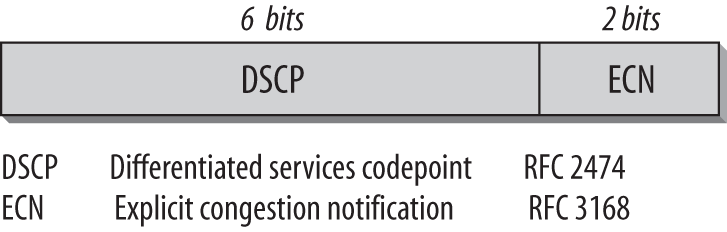
\includegraphics[width=250px]{figures/trafficclass.png}
    \centering
    \caption{Structure du champ Traffic Class. \cite{Hagen2014}}
    \end{figure}
	
    
    Les 6 premiers bits définissent la valeur du DSCP  qui détermine la gestion des priorités du traffic ou per-hop behavior (PHB) de chaque routeur. 
    
    Le PHB détermine comment les paquets seront transmis par le routeur.
    Le PHB par défaut est codé par la suite : 000000. Il correspond au best-effort forwarding behavior c.a.d. que le réseau transmettra ces paquets sans aucune priorité et utilisera les ressources disponibles pour les transmettre.
    
    \begin{table}[!h]
  \centering
  \begin{tabular}{|l|l|l|} 
   \hline
    Groupe & Format du Codepoint & Politique d'affectation\\
    \hline
    1 & xxxxx0 & Usage standard \\
    \hline
    2 & xxxx11 & Usage expérimental ou local\\
    \hline
    3 & xxxx01 & Usage expérimental ou local; Ou en complément du groupe 1\\
    \hline
  \end{tabular}
  \caption{Groupes de Codepoints.}
\end{table}

    3 groupes de Code Points sont définis : xxxxx0 pour des PHB standardisés, xxxx11 pour un usage expérimental ou local et xxxx01 pour un usage expérimental ou local ou en supplément du groupe xxxxx0 si il est entièrement utilisé.
    
    Les 2 derniers bits du champ Traffic Class sont utilisés pour la notification explicite de congestion (ECN). Ces bits sont présents dans IPv4 et IPv6.

\subsection{Le champ HopByHop}
    Le champ HopByHop dans l'entete des options peut aussi être utilisé pour transporter un message d'alerte routeur (Multicast Listener Discovery message, RSVP message....). De cette manière, le paquet peut être traité plus rapidement car il est inutile d'analyser des entetes d'autres protocoles de plus haut niveau par les routeurs intermédiaires pour détecter que c'est un paquet message.
    
\subsection{Absence de NAT}
	La Network Address Translation (NAT) n'existe plus en IPv6 car suffisament d'adresses IP sont disponibles et donc la NAT n'est plus nécessaire. De cette manière, la QoS n'est plus arrêtée par la NAT et peut s'étendre sur des réseaux plus importants.
\chapter{Expérimentation}\label{ch:experimentation}

	La partie expérimentation de notre projet concerne principalement le test de la qualité de service (QoS). Néanmoins, nous avons dû apprendre à utiliser le routeur et à le configurer avant de pouvoir réaliser nos tests. 

\section{Connexion au routeur}

	Pour configurer le réseau nous avons dû nous connecter au routeur via l'utilitaire Putty par le port serial<->USB. De cette manière, on accède à l'interface de configuration Cisco en ligne de commande.

            \begin{figure}[h]
            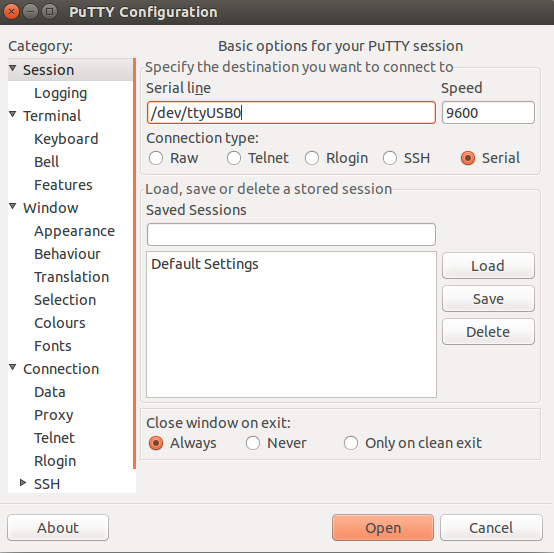
\includegraphics[width=250px]{figures/putty.png}
            \centering
            \caption{Connexion de notre ordinateur au routeur}
            \end{figure}
           
\section{Configuration du routeur}
    
	\subsection{Configuration du vlan}
    
    	Avant de connecter nos machines, il faut créer un vlan (Virtual Local Area Network) pour pouvoir utiliser IPv6. En effet, il est impossible d'activer directement l'IPv6 sur les interfaces FastEthernet 1 à 7 avec le modèle de routeur dont nous disposons.
        
    	On crée ici un vlan appelé "vlan 2" :
        \begin{lstlisting}[frame=single]
              vlan database
              vlan 2
        \end{lstlisting}
\newpage
	\subsection{Configuration des interfaces}
        	
		On configure ensuite les différentes interfaces du routeur que l'on va utiliser (fastEthernet 1 à 3 pour notre expérimentation). 
    
Exemple de la configuration de l'interface 1 :
        \begin{lstlisting}[frame=single]
            interface FastEthernet 1
            switchport mode access
            switchport access vlan 2
        \end{lstlisting}
    
    On précise que l'interface est prête à recevoir des informations avec "mode access" et qu'elle est liée au vlan 2.
    
	\subsection{Configuration IPv6}
        
        On passe en mode configuration pour l'interface du vlan 2 et on lui attribue une adresse IPv6. 
        
        On affecte à chaque machine du vlan 2 une adresse générée à partir du préfixe 2001:DB8:0:1::/64 et de l'adresse MAC de la machine (option eui-64).
        
        Configuration :
        \begin{lstlisting}[frame=single]
          interface vlan 2
          ipv6 address 2001:DB8:0:1::/64 eui-64
          ipv6 enable
          no ip address
          exit
          ipv6 unicast-routing 
        \end{lstlisting}
        
        À noter que l'on a désactivé l'adressage IPv4 avec la commande suivante afin d'être certain que nos services utilisent l'IPv6 :
        \begin{lstlisting}[frame=single]
			no ip address
        \end{lstlisting}
        
	\subsection{Test de la connexion et adressage IPv6}
        
        Une fois que la configuration IPv6 est effectuée, on connecte nos ordinateurs sur les interfaces puis on teste la connexion.
        
        Tout d'abord on vérifie qu'une adresse IPv6 a été affectée à chaque machine connectée au routeur.
Pour cela on utilise la commande suivante :

        \begin{lstlisting}[frame=single]
			ifconfig
        \end{lstlisting}
        
        \begin{figure}[h]
        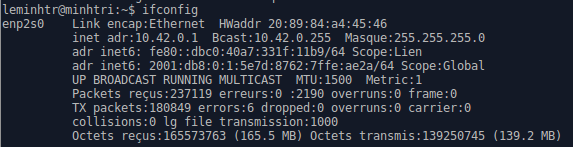
\includegraphics[width=250px]{figures/ipv6-adr.png}
        \centering
        \caption{Résultat de la commande ifconfig}
        \end{figure}
        
        On peut voir une adresse IPv6 link-local en FE80:, qui a été automatiquement affectée à la machine par défaut.
        On a également l'adresse unicast global commençant par 2001:DB8:0:1 (préfixe) suivi d'une adresse dérivée de l'adresse MAC de la machine.
        
        L'adresse multicast FF02::1 est aussi disponible par défaut, toutes les machines du LAN écoutent à cette adresse.
        L'adresse FF02::2 désigne quant à elle tous les routeurs du LAN.
        
         On teste également la connexion entre le routeur et l'ordinateur en effectuant un ping (requête ICMP echo).
            \begin{figure}[h]
            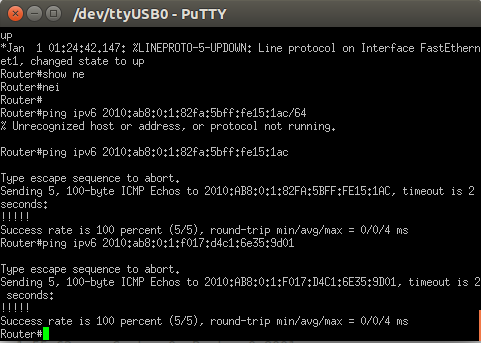
\includegraphics[width=250px]{figures/pings2.png}
            \centering
            \caption{On ping la machine depuis le routeur}
            \end{figure}

            \begin{figure}[h]
            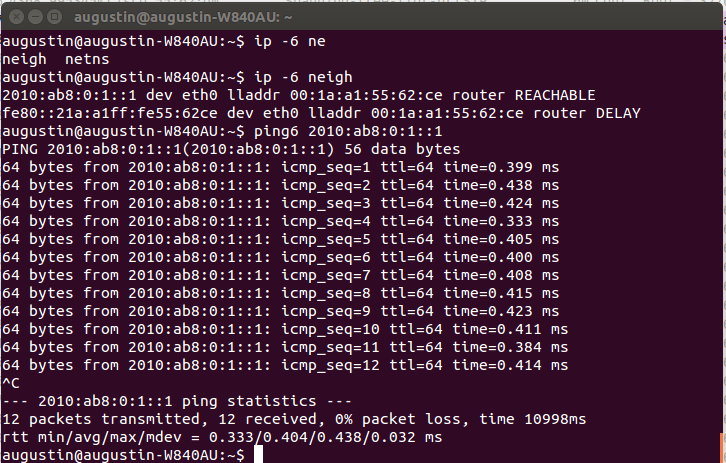
\includegraphics[width=250px]{figures/pings.png}
            \centering
            \caption{Ping depuis la machine vers le routeur}
            \end{figure}
        
    La connexion fonctionne correctement car aucun paquet n'est perdu !
    
    On peut également tester un ping sur l'adresse multicast FF02::1, en précisant l'interface de sortie, de cette manière dans un terminal :
    	\begin{lstlisting}[frame=single]
ping6 -I eth0 FF02::1
        \end{lstlisting}
     Cela permet de connaître tous les clients connectés au routeur.
    
	\subsection{Sauvegarde des différentes configurations du routeur}
    
    \subsubsection{Problème avec le chargement de le configuration de démarrage}
    
    	Nous avons rencontré un problème avec le chargement de la startup-config lorsqu'on démarre notre routeur. En effet, le mode de paramétrage du routeur faisait qu'au démarrage, la configuration n'était pas chargée depuis startup config. Nous avons donc corrigé ce problème de la manière suivante. 
    
Le paramètre de configuration registre est un code hexadécimal qui permet de changer le comportement du routeur au démarrage.\cite{config-register} Notamment : 
\begin{itemize}
\item comment le routeur démarre (ROMmon, NetBoot)
\item avec quelles options (ignorer la configuration de démarrage, désactiver les messages de démarrage)
\item la vitesse de la console (en bauds)
\end{itemize}
        
La commande :         
		\begin{lstlisting}[frame=single]
          show version
        \end{lstlisting}
permet de connaître le code du paramètre de configuration registre (dernière ligne du résultat).

Le code de paramètre de configuration registre présent à l'origine était le 0x2142 qui configure le routeur pour ignorer la configuration de démarrage (startup-config). 
Nous avons redéfini le code de paramètre de configuration registre à sa valeur par défaut sortie d'usine : 0x2102, ce qui permet de charger la configuration de démarrage au démarrage.
        
        \begin{lstlisting}[frame=single]
          show version
          conf t
          config-register 0x2102
        \end{lstlisting}
        
	    \begin{figure}[h]
        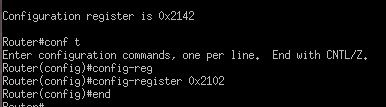
\includegraphics[width=250px]{figures/config-register_0x2102.png}
        \centering
        \caption{Modification du paramètre de configuration}
        \end{figure}

	\subsubsection{Sauvegardes et changements de configurations}

		Nous avons sauvegardé différentes configurations du routeur (avec et sans QoS) dans des fichiers sur la carte compact flash du routeur, par exemple dans le fichier SR04QOS : 
        \begin{lstlisting}[frame=single]
          copy running-config SR04QOS
        \end{lstlisting}
        
        Pour changer de configuration (passer d'une configuration sans QoS à une configuration avec QoS par exemple), on copie le fichier de configuration de la carte dans la startup-config puis on recharge la configuration du routeur :
        
        \begin{lstlisting}[frame=single]
            copy SR04QOS startup-config
            reload
        \end{lstlisting}


    \section{Mise en place des services}
    
    Pour tester la qualité de service, nous avons mis en place quelques services pour tester la connexion. Nous nous sommes concentrés sur les logiciels de voix sur IP puis par la suite, nous avons fait du streaming vidéo. 
    
    Note : Les services ont été mis en place sur un ordinateur utilisant ArchLinux (gestion de service : systemctl). Les configurations des serveurs et les procédures d'installation ne sont pas présentées ici car hors-sujet.
    
	\subsection{Conférence audio}
    
    	Nous avons installé et hébergé un serveur Murmur sur une de nos machines. Murmur permet d'héberger des salons de discussions (conversation vocale et écrite) du logiciel Mumble. Mumble est un logiciel permettant la voix sur IP, et permet donc de communiquer oralement à distance. 

Il faut d'abord se connecter au serveur Murmur que nous avons créé. L'adresse est l'adresse IPv6 de l'ordinateur faisant tourner le serveur.
        \begin{figure}[h]
        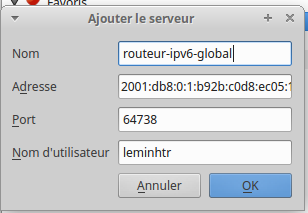
\includegraphics[width=250px]{figures/mumble-config.png}
        \centering
        \caption{Connexion au serveur Murmur dans Mumble}
        \end{figure}
        
Il est également possible d'activer/désactiver la QoS sur Mumble, fonctionnalité utile pour nos tests.

        \begin{figure}[h]
        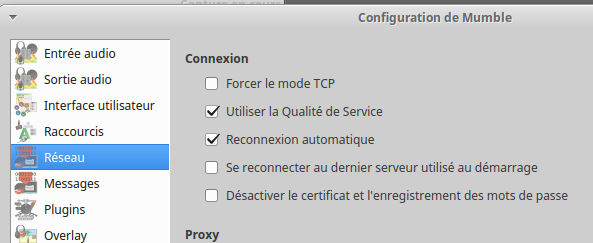
\includegraphics[width=250px]{figures/qos-mumble-config2.png}
        \centering
        \caption{Option QoS de Mumble}
        \end{figure}


Enfin, nous avons réussi à discuter par message écrit et VoIP (une bouche est rouge quand une personne parle par VoIP)

        \begin{figure}[h]
        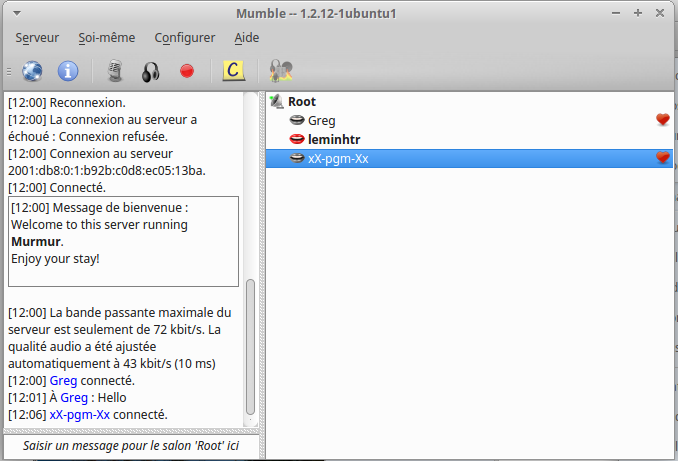
\includegraphics[width=250px]{figures/qos-mumble-talk.png}
        \centering
        \caption{Salon de discussion Mumble (3 personnes)}
        \end{figure}
        
\newpage
        
	\subsection{Transfert de fichier}
        Nous avons installé et hébergé un serveur SSH pour le transfert de fichier en SFTP (openSSH).

		\begin{figure}[!h]
          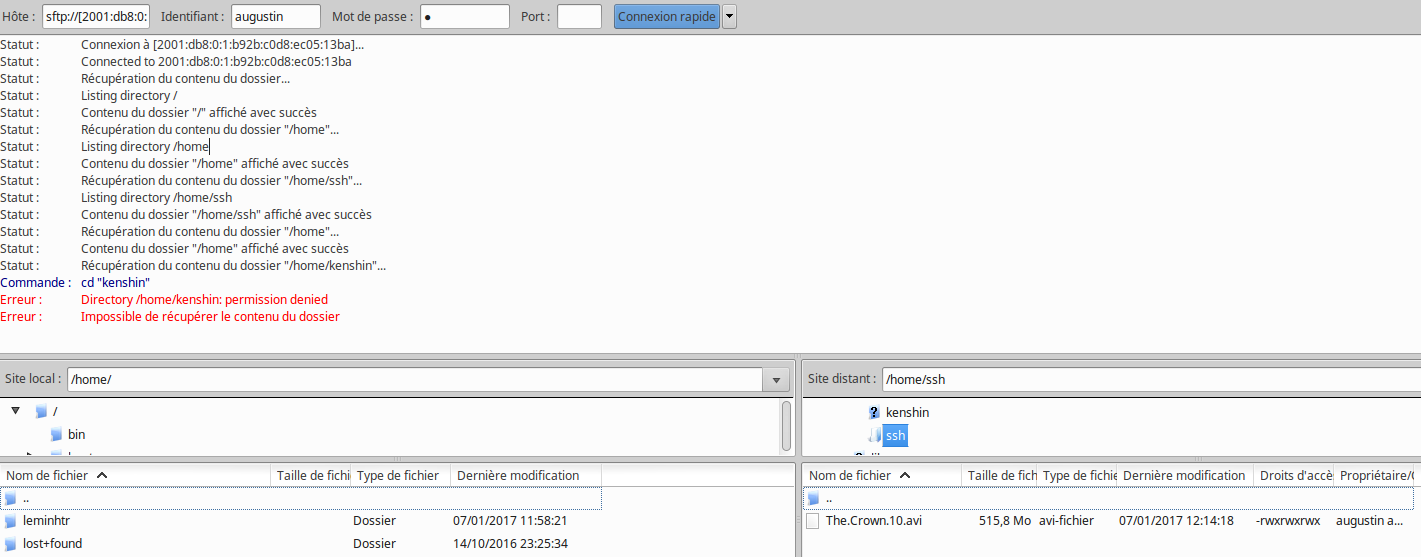
\includegraphics[width=400px]{figures/filezilla.png}
          \centering
          \caption{Configuration et accès au serveur SSH}
        \end{figure}

	\subsection{Téléphonie}
    
    Bien que nous ayons déjà pu tester la VoIP avec Mumble, nous voulions voir ce que cela donnait avec des téléphones. Nous avons donc emprunté deux téléphones utilisant la VoIP fournis par le département du GI.
    
    Le téléphone possède deux méthodes d'alimentation possible : PoE (Power over Ethernet) ou par alimentation classique (Transformateur 220v -> 36V).
    Le POE permet de transmettre à un équipement à la fois des données, mais aussi son alimentation électrique via le câble Ethernet, deux des quatre paires du câble sont allouées à l'alimentation électrique. Cette technique permet d'éviter l’installation d’un double réseau (IP et électrique). Cependant, le routeur ne dispose pas de l'option facultative permettant le support de la PoE. L'alimentation s'est donc faite via transformateur.
    
    La mise en place du téléphone fut assez longue : nous avons dû lire la documentation technique pour téléphone. La mise en place de 4 serveurs (TFTP, FTP, HTTP, SIP) ainsi qu'une configuration assez complète, notamment pour la gestion du protocole SIP. Nous avons appris par ce biais à mettre en place une architecture VOIP complète qui nous a permis de passer des appels entre tous nos différents appareils : téléphone portable (via Linphone), ordinateur (via Ekiga) et bien sûr, via le téléphone IP.
    
   
	\subsection{Vidéo à la demande, streaming}
    
    	Nous avons implémenté un serveur HTTP afin de pouvoir faire du streaming vidéo.
        \begin{lstlisting}[frame=single]
vlc -vvv '/home/ssh/film.avi' --ipv6 --sout'#
transcode{vcodec=h264,acodec=mpga,ab=128,channels=2,
samplerate=44100}:http{mux=ffmpeg{mux=flv},dst=:8080/SR04}'
--ttl 12 --sout-all 
        \end{lstlisting}
        
        \begin{figure}[!h]
        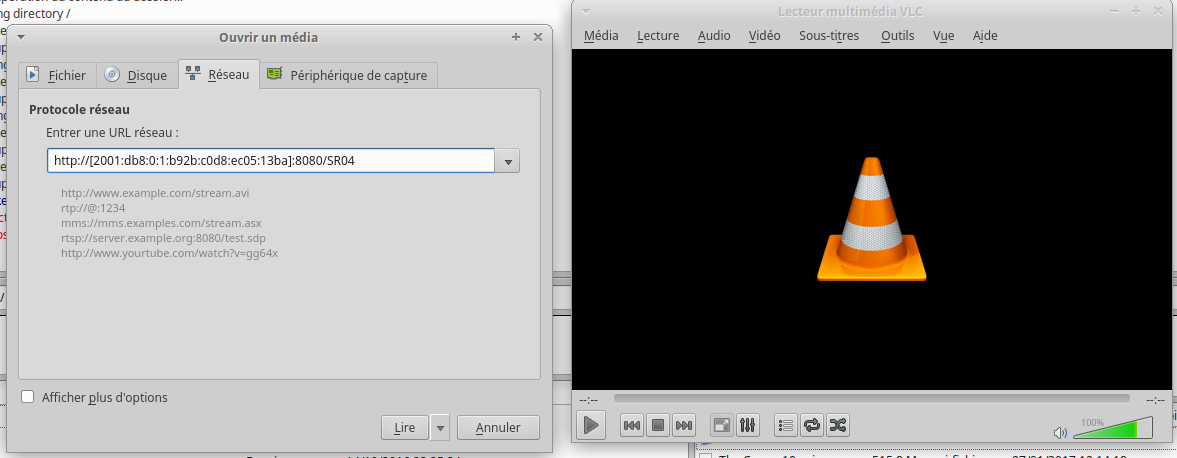
\includegraphics[width=400px]{figures/qos-vlc-config.png}
        \centering
        \caption{Configuration de l'accès au streaming}
        \end{figure}

        \begin{figure}[h]
        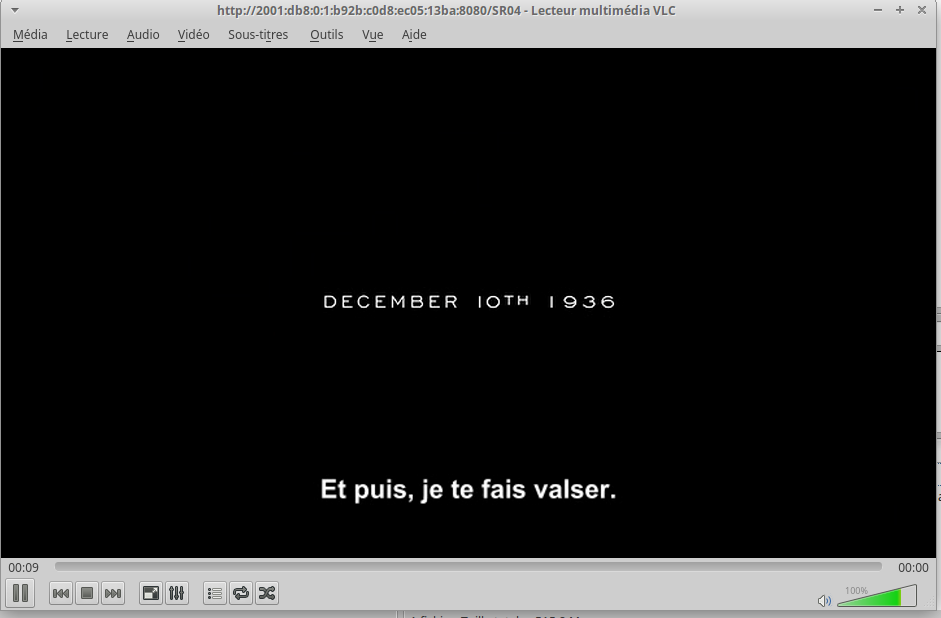
\includegraphics[width=250px]{figures/qos-vlc-stream.png}
        \centering
        \caption{Streaming d'une vidéo}
        \end{figure}

   Au cours de nos différents essais de streaming, nous avons également essayé le protocole RTP (Real-time Transport Protocol) et son homologue gérant la qualité de service : le protocole RTCP (RTP Control Protocol). RTCP sert à s'assurer de la qualité de service et permet de synchroniser les flux. Pour utiliser ces protocoles, nous avons dû créer et utiliser un groupe multicast. 
    
%%%%%%%%%%%%%%%%%%%%%%%%%%%%%%%%%%%%%%%%%%%%%%%%%%%%%%
    \section{Mise en place de la qualité de service}

		Pour mettre en place notre qualité de service, nous nous sommes basés sur les services différenciés (DS - Differentiated Services), expliqués section \ref{diffserv}. Ce type de QoS utilise le champ Traffic Class d'un paquet IPv6 afin de préciser le DSCP (Differentiated Services Code Point). Le DSCP est un code permettant de classifier et de gérer les paquets d'un réseau suivant une certaine priorité. Ainsi, on peut demander au routeur d'accélérer au maximum le passage de certains paquets en précisant le code DSCP "EF" dans leur champ Traffic Class. Cette QoS est gérée au niveau de chaque routeur, suivant leur politique de traitement des paquets. Lorsqu'aucun code DSCP n'est entré, le routeur applique une politique par défaut : "best effort".

		Ci-dessous se trouvent les instructions permettant d'implémenter la qualité de service.

		%%%%%%%%%%%%%%%%%%%%%%%%%%%%%%%%%%%%%%
		\subsection{Configuration d'une classe}
        
        Supposons que l'on veuille donner la priorité aux paquets échangés entre un serveur Http et un ordinateur, sur le port 80.
        
        En utilisant la commande ci-dessous, on crée un groupe d'accès appelé 100. Ce groupe va référencer les paquets provenant du port 80 (eq 80) de n'importe quelle source (premier any) vers n'importe quelle destination (second any). 
        \begin{lstlisting}[frame=single]
access-list 100 permit tcp any any eq 80
        \end{lstlisting}
        
        On crée ensuite une classe nommée "http". Une classe permet de représenter un ensemble de paquets sur lesquels on va appliquer une politique de traitement. La commande "match..." permet donc de spécifier les conditions d'appartenance à la classe. Ici, il faut que le paquet soit dans le groupe 100. 
        \begin{lstlisting}[frame=single]
class-map http
match access-group 100
        \end{lstlisting}
         
        %%%%%%%%%%%%%%%%%%%%%%%%%%%%%%%%%%%%%%%
        \subsection{Configuration d'une politique de traitement des paquets}

		Une fois que l'on connaît les paquets sur lesquels appliquer la QoS, il ne reste plus qu'à préciser la politique de traitement. 
        Ici, on crée une politique nommée "acceshttp" qui s'appliquera à la classe "http". On précise ensuite la priorité que l'on donne aux paquets avec "set dscp". 
		\begin{lstlisting}[frame=single]
policy-map acceshttp 
class http
set dscp cs4
        \end{lstlisting}
       
        Il ne reste plus qu'à ajouter la politique de traitement au vlan. "output" permet de préciser si le traitement se fait en entée ou en sortie du routeur. 
        \begin{lstlisting}[frame=single]
interface vlan 2 
service-policy output acceshttp
        \end{lstlisting}

		De cette manière, les paquets allant vers le port 80 auront leur champ DSCP à cs4. Ils seront prioritaires sur les autres ! Attention tout de même lorsqu'on précise un DSCP, il existe une hiérarchie entre les différents codes. Certains seront prioritaires sur d'autres.
        
        Il est possible de préciser beaucoup plus de conditions au niveau des classes. On peut conditionner les paquets suivant leur adresse IP, suivant un protocole utilisé (RTP par exemple)...
        
        De même, on peut réaliser des politiques de traitement plus poussées, en allouant par exemple un pourcentage de la bande passante aux paquets d'une classe.
        
        L'ensemble de méthode de tri (class-map) et des politiques (policy) sont disponibles ici \url{https://www.cisco.com/c/en/us/td/docs/ios/12_2/qos/configuration/guide/fqos_c/qcfmcli2.html}

%%%%%%%%%%%%%%%%%%%%%%%%%%%%%%%%%%%%%%%%%%%%%%%%%%%%%%
    \section{Test de la qualité de service}
    
    %%%%%%%%%%%%%%%%%%%%%%%%%%%%%%%%%
    \subsection{Saturation du réseau}
       
    Pour tester la QoS, nous avons cherché à saturer le réseau. Pour cela, nous avons fait du streaming d'une vidéo 1080p sur deux postes. La vidéo reçue par le poste de droite \ref{vlc-compar} a des difficultés à s'afficher en temps réel (problème de Codec, la charge sur le réseau reste la même).
		\begin{figure}[h]
        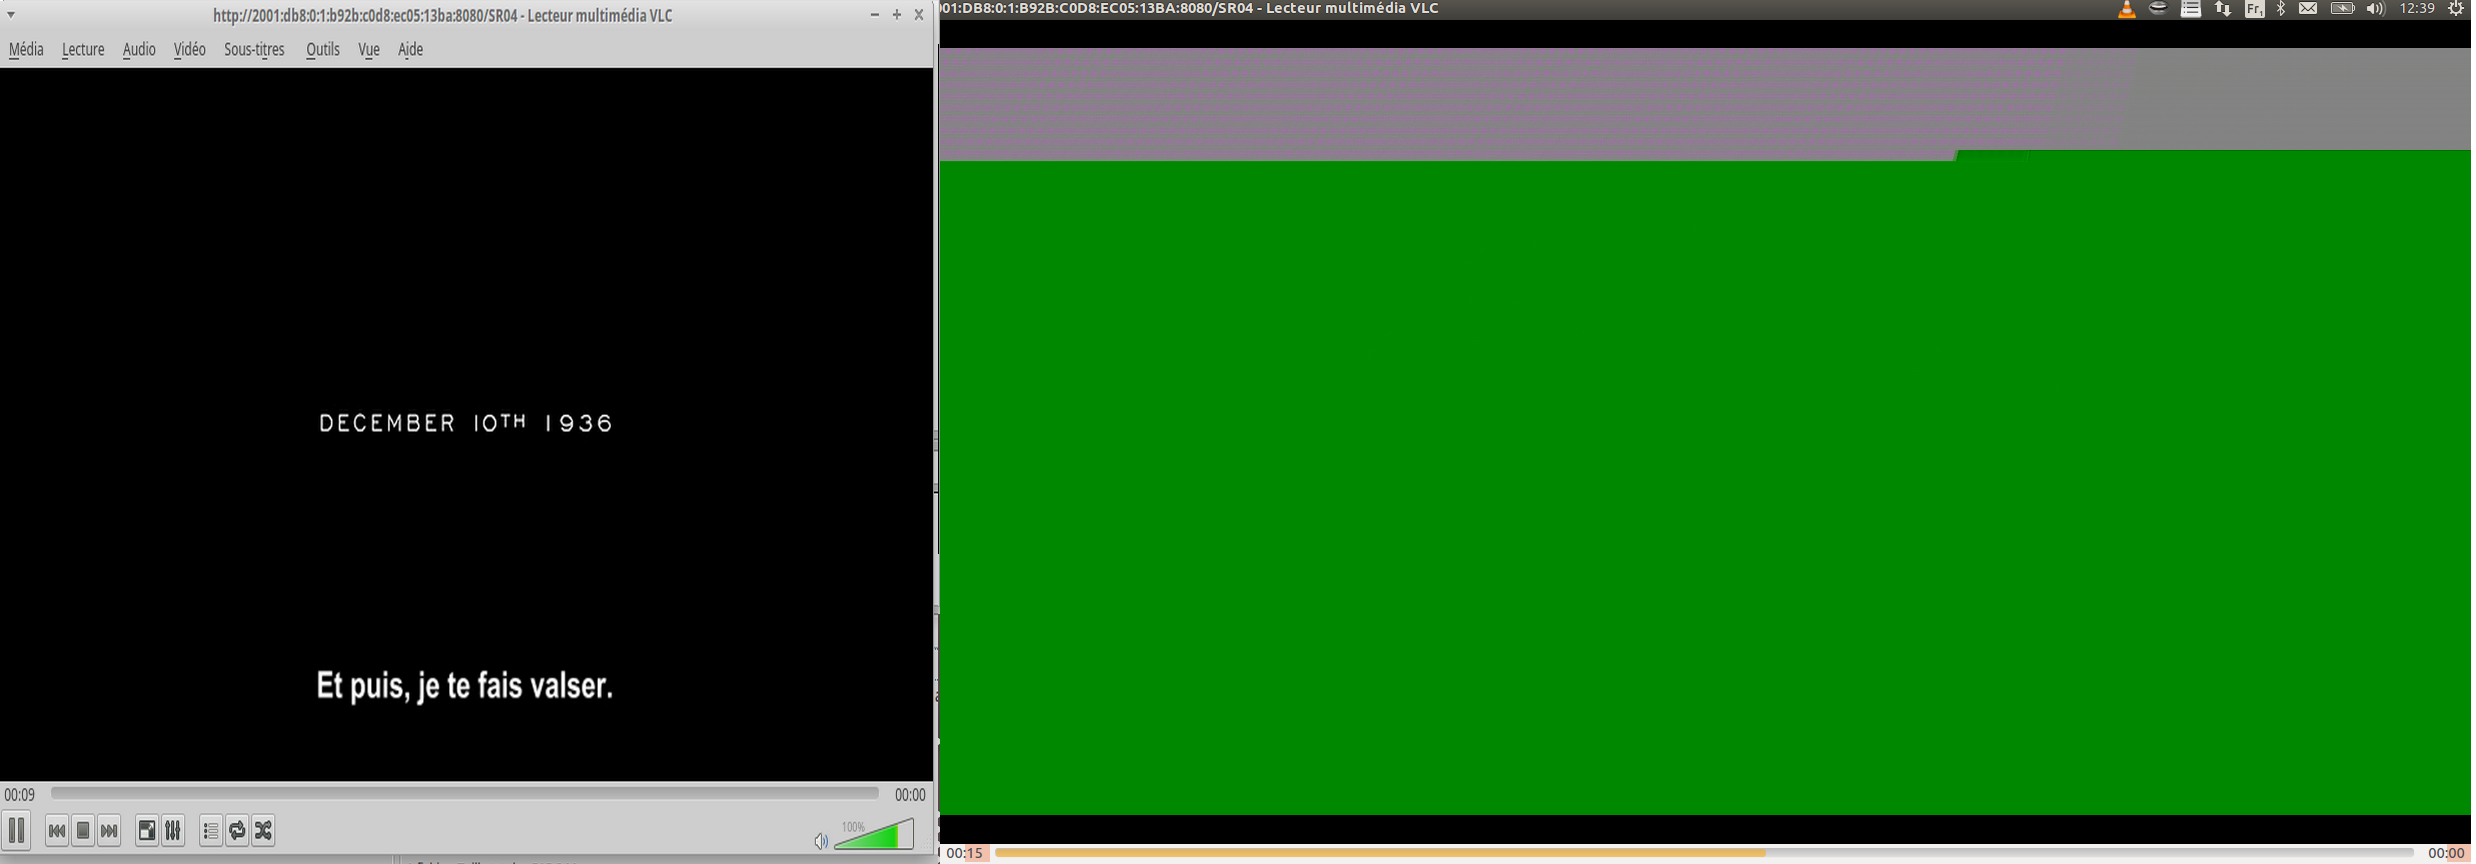
\includegraphics[width=400px]{figures/vlc-stream-compar.png}
        \centering
        \caption{Streaming d'une vidéo par 2 postes}
        \label{vlc-compar}
        \end{figure}
	
    Pendant la saturation du réseau, nous avons tenté de passer un appel VOIP sur Mumble. La latence était importante et la qualité mauvaise. Le besoin de la QoS se faisait ressentir.
      
    %%%%%%%%%%%%%%%%%%%%%%%%%%%%%%%%%%%
    \subsection{Test de la QoS par Ping}
    
    Pour prouver le bon fonctionnement de la QoS, nous avons trouvé une méthode se servant de l'utilitaire ping. Nous avons ensuite observé les paquets sur Wireshark. 
    
    La commande suivante permet d'envoyer un paquet en spécifiant le ToS(Type of Service) souhaité. Le ToS est un code comprenant le DSCP. On peut l'obtenir par la formule DSCP*4 = TOS, ou par des tables de conversion comme celle-ci : \cite{TOSDSCP}.
        \begin{lstlisting}[frame=single]
ping6 -Q <ToS> <adresse IP>
ping6 -Q 0x68 fe80::4ab9:ab2:77dd:ee4c%en3
        \end{lstlisting}  
  
    L'idée du test est donc d'activer la QoS au niveau du routeur et de charger le réseau en envoyant un fichier très lourd par exemple. On envoie ensuite un ping pour vérifier que la valeur DSCP entrée n'est pas perdue en cours de route. On peut voir cela avec Wireshark, qui repère le champ correspondant au DSCP et la priorité fixée. On peut également vérifier l'impact de la QoS entre un ping normal et un ping spécifiant le DSCP. On utilise la priorité EF, Expedited Forwarding, améliorant le temps d'acheminement du paquet.
    
        \begin{figure}[h]
        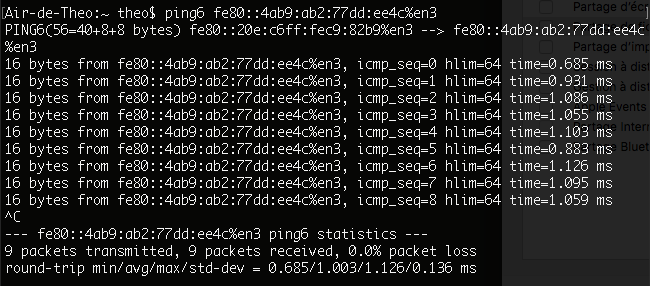
\includegraphics[width=350px]{figures/ping_sans_qos.png}
        \centering
        \caption{Envoie d'un ping sans QoS}
        \end{figure}
        
        \begin{figure}[h]
        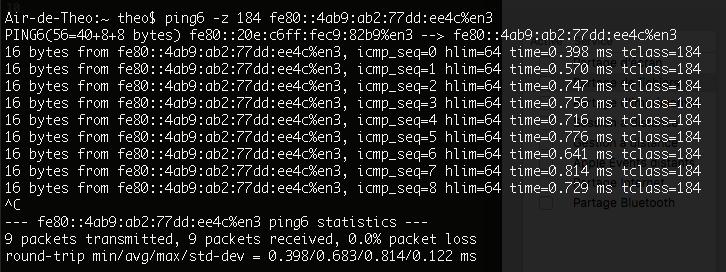
\includegraphics[width=350px]{figures/ping_qos.png}
        \centering
        \caption{Envoie d'un ping avec QoS}
        \end{figure}
        
    Petite remarque, la commande est ici ping6 -Z car elle a été réalisée sur Mac OS.
    
    En moyenne le ping met 1.003 ms pour arriver sans QoS et 0.683 ms avec QoS.
    
    Cela représente donc une amélioration de 68\% (0.683/1.003) du temps d'acheminement.
      
    On a choisi les codes DSCP correspondants au téléphone VoIP que nous avions afin de passer le Per-Hop Behavior des paquets de notre téléphone en AF, alors que tous les autres paquets étaient en default. La téléphonie VoIP devient donc prioritaire.
    
    %mettre tous les screens wireshark
    Pour le code DSCP : EF, le Per-Hop Behavior est EF (Expedited Forwarding).
    Le routeur met en priorité les ressources nécessaires pour réduire les délais, la gigue, les pertes par un service de bout en bout. Cela est très utile pour assurer le trafic temps-réel des applications telles que la VoIP ou le streaming vidéo. Il y a cependant une limite concernant le nombre de paquets marqué par un code DSCP à EF pour limiter la surcharge et les délais.
    
    Nous avons effectué un ping avec EF (Les bits DSCP sont à 46 en décimal.).
        \begin{figure}[h]
        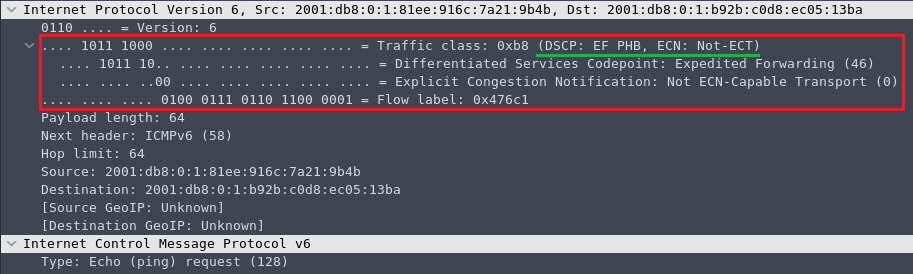
\includegraphics[width=350px]{figures/dscp-ef-color.png}
        \centering
        \caption{Expedited Forwarding PHB}
        \end{figure}
        
	Pour le code DSCP : AF31, le Per-Hop Behavior est AF (Assured Forwarding).
    Dans ce cas, l'émetteur est assuré de la réception tant que la congestion du réseau n'est pas trop significative. Une partie de la bande passante est garantie et les classes d'AF peuvent avoir accès à un supplément si possible. Il existe plusieurs classes d'AF (\ref{af_class}). Elles se distinguent par des niveaux de priorité croissant (Classe) et la probabilité de perte (Faible, moyenne, haute).
        \begin{figure}[h]
        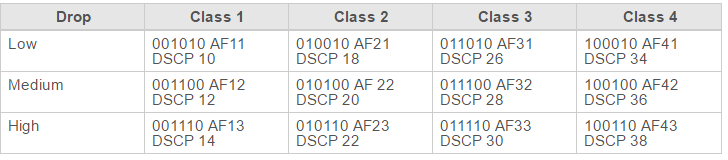
\includegraphics[width=350px]{figures/dscp_af-class.PNG}
        \centering
        \caption{Classe d'AF}
        \label{af_class}
        \end{figure}
\newpage        
        Nous avons ici effectué un ping avec AF31, cela correspond donc à une classe 3 avec une faible probabilité de perte.
        \begin{figure}[h]
        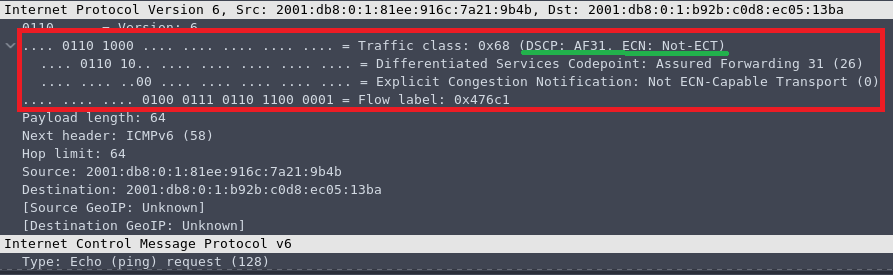
\includegraphics[width=350px]{figures/dscp-af-color.png}
        \centering
        \caption{Assured Forwarding PHB}
        \end{figure}
        
       
    Pour tous les autres codes : le Per-Hop behavior est default. Le comportement est alors \textit{"Best Effort"}.
		\begin{figure}[h]
        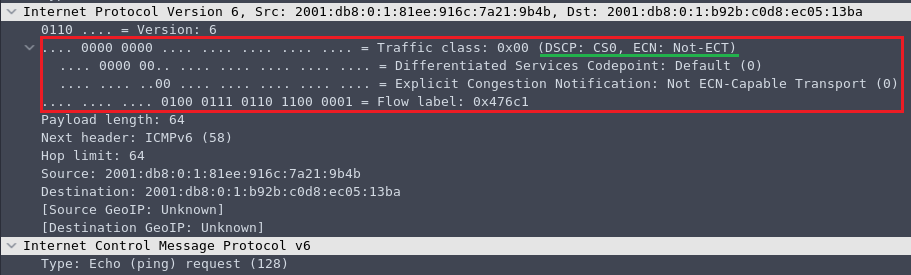
\includegraphics[width=350px]{figures/dscp-dflt-color.png}
        \centering
        \caption{Default PHB}
        \end{figure}
        
 	%%%%%%%%%%%%%%%%%%%%%%%%%%%%%%%%%%%%%%%
    \subsection{Test de la QoS par l'essai}
    
	Une fois la QoS fonctionnelle, nous avons recommencé l'expérience de départ : Streaming d'une vidéo 1080p sur deux ordinateurs. Lorsque le réseau était saturé, nous avons tenté un appel VOIP. Cette fois-ci, c'est la vidéo qui était ralentie. L'appel ne présentait aucune latence. 
    L'objectif de la QoS était atteint : c'est l'appel VOIP qui était prioritaire sur le streaming vidéo.
  	
    
    
    
    
    
    
    
\chapter{Conclusion}\label{ch:conclusion}

Ce projet expérimental dans le cadre de l'UV SR04 fut riche en apprentissage de nouvelles connaissances théoriques et pratiques pour l'ensemble de notre groupe de projet. 

Nous avons pu revoir en détail la théorie du modèle OSI (Open Systems Interconnection) et le fonctionnement de sa couche réseau (couche 3). Nous avons également parlé des spécificités du routage et avons étudié en détail différents protocoles de la couche réseau :  l'IPv6, l'ICMPv6. Nous avons su montrer quelles sont les nouveautés et avantages apportés par la norme IPv6 par rapport à la norme IPv4.

Nous avons ensuite présenté dans notre rapport les grands principes et mises en œuvre de la Qualité de Service (QoS) qui était le sujet central de notre étude.

Une fois l'étude théorique bien avancée, nous avons pu commencer à tester en pratique les principes étudiés précédemment en théorie. Il nous a fallu pour cela apprendre à configurer et manipuler les fonctionnalités de base d'un routeur Cisco. Puis nous avons mis en fonctionnement et testé le routage, l'adressage, l'autoconfiguration en IPv6 sur ce routeur.

Finalement, nous avons mis en place des configurations du routeur avec et sans QoS. Puis nous avons tenté de saturer le routeur en créant du trafic à l'aide de plusieurs machines et plusieurs applications (conférence audio, transfert de fichier, téléphonie, streaming vidéo) le tout de manière simultanée.

Ces tests expérimentaux, mettant en place la QoS pour les services de VoIP, nous ont permis d'apprendre à installer une QoS simple dans un réseau et à démontrer l'efficacité de la QoS dans le but de favoriser certaines applications dans une architecture réseau.

Nous tenons particulièrement à remercier M. Bouabdallah et l'équipe pédagogique de l'UV SR04 pour leur soutien, leur aide et leurs conseils apportés tout au long du projet.


\nocite{Couchereseaux}
\nocite{Rout_vecteur}
\nocite{Algo_routage}
\nocite{Xripng}
\nocite{Xospf}
\nocite{RFC}
\nocite{Shichao}
\printbibliography[heading=bibintoc]
\label{bib:mybiblio}
\end{document}